% !TEX TS-program = pdflatex
% !TEX encoding = UTF-8 Unicode

% This is a simple template for a LaTeX document using the "article" class.
% See "book", "report", "letter" for other types of document.

\documentclass[11pt, titlepage]{article} % use larger type; default would be 10pt

\usepackage[utf8]{inputenc} % set input encoding (not needed with XeLaTeX)

%%% Examples of Article customizations
% These packages are optional, depending whether you want the features they provide.
% See the LaTeX Companion or other references for full information.

%%% PAGE DIMENSIONS
\usepackage{geometry} % to change the page dimensions
\geometry{a4paper} % or letterpaper (US) or a5paper or....
\geometry{margin=2cm, headsep=5mm, includefoot, includehead}

\usepackage{graphicx} % support the \includegraphics command and options
\graphicspath{{figures/}} % Location of the graphics files
% \usepackage[parfill]{parskip} % Activate to begin paragraphs with an empty line rather than an indent

%%% PACKAGES
\usepackage{booktabs} % for much better looking tables
\usepackage{array} % for better arrays (eg matrices) in maths
\usepackage{paralist} % very flexible & customisable lists (eg. enumerate/itemize, etc.)
\usepackage{verbatim} % adds environment for commenting out blocks of text & for better verbatim
\usepackage{subfig} % make it possible to include more than one captioned figure/table in a single float
% These packages are all incorporated in the memoir class to one degree or another...

%%% HEADERS & FOOTERS
\usepackage{fancyhdr} % This should be set AFTER setting up the page geometry
\pagestyle{fancy} % options: empty , plain , fancy
\fancyhead{}
%%% SECTION TITLE APPEARANCE
\usepackage{sectsty}
\allsectionsfont{\sffamily\mdseries\upshape} % (See the fntguide.pdf for font help)
% (This matches ConTeXt defaults)

%%% ToC (table of contents) APPEARANCE
\usepackage[nottoc,notlof,notlot]{tocbibind} % Put the bibliography in the ToC
\usepackage[titles,subfigure]{tocloft} % Alter the style of the Table of Contents
\renewcommand{\cftsecfont}{\rmfamily\mdseries\upshape}
\renewcommand{\cftsecpagefont}{\rmfamily\mdseries\upshape} % No bold!

\usepackage{lastpage}
\usepackage{rotating}
\usepackage{textcomp} %get the correct micro sec display
\usepackage{float}
%---------- Enable IEEEtran.bst configurations ------
\usepackage{IEEEtrantools}
\usepackage{verbatim}
%----------------------------------------------------

%%% END Article customizations

%%% The "real" document content comes below...

%%% Header %%%%%%%%%%%%%%%%%%%%%%%%%%%%%
\setlength{\headheight}{53pt}
\lhead{MF2063 Embedded Systems Design Project \\		 
       ESS-NW/ESS-CAR \\
       Leon Fernandez, leonfe@kth.se}
\rhead{Final Report \\
       Version 1 \\
       \thepage(\pageref{LastPage})}
\renewcommand{\headrulewidth}{1pt}
%%%%%%%%%%%%%%%%%%%%%%%%%%%%%%%%%%%%%%%%

%%% Footer %%%%%%%%%%%%%%%%%%%%%%%%%%%%%
%\cfoot{blablablabla}
%\renewcommand{\footrulewidth}{0.4pt}
%%%%%%%%%%%%%%%%%%%%%%%%%%%%%%%%%%%%%%%%
%\date{} % Activate to display a given date or no date (if empty),
         % otherwise the current date is printed 

\begin{document}
%\maketitle
\bstctlcite{BSTcontrol} % IEEEtran.bst controls enabled


%----------------------------------------------------------------------------------------
%	TITLE PAGE
%----------------------------------------------------------------------------------------

\begin{titlepage} % Suppresses displaying the page number on the title page and the subsequent page counts as page 1
	\newcommand{\HRule}{\rule{\linewidth}{0.5mm}} % Defines a new command for horizontal lines, change thickness here
	
	\center % Centre everything on the page
	
	%------------------------------------------------
	%	Headings
	%------------------------------------------------
	
	\begin{figure}
   		\centering
    	
\includegraphics[scale=1]{kthLogo.png}
	\end{figure}
	
	\textsc{\LARGE KTH Mechatronics Advanced Course}\\[1cm] % Main heading such as the name of your university/college
	
	\textsc{\Large MF2063, HT 2018}\\[0.5cm] % Major heading such as course name
	
	\textsc{\Large FINAL REPORT}\\[0.5cm] % Major heading as well
	
	%------------------------------------------------
	%	Title
	%------------------------------------------------
	
	\HRule\\[0.4cm]
	
	{\huge\bfseries ESS-NW/ESS-CAR}\\[0.4cm] % Title of your document
	
	\HRule\\[1.5cm]	
	
	%------------------------------------------------
	%	Author(s)
	%------------------------------------------------
	
	\begin{minipage}{0.4\textwidth}
		\begin{flushleft}
			\large
                        \textsc{Jonas Ekman}
			\\
			\textsc{Yini Gao}
                        \\
                        \textsc{Jacob Kimblad}
		\end{flushleft}
	\end{minipage}
	~
	\begin{minipage}{0.4\textwidth}
		\begin{flushright}
			\large
                        \textsc{Leon Fernandez}
			\\
			\textsc{Fredrik Hyyrynen}
                        \\
                        \textsc{Yifan Ruan}
		\end{flushright}
	\end{minipage}
	
	% If you don't want a supervisor, uncomment the two lines below
        % and comment the code above
	%{\large\textit{Author}}\\
	%John \textsc{Smith} % Your name
	\vskip 8cm
	\begin{figure}[H]
   		\centering
    	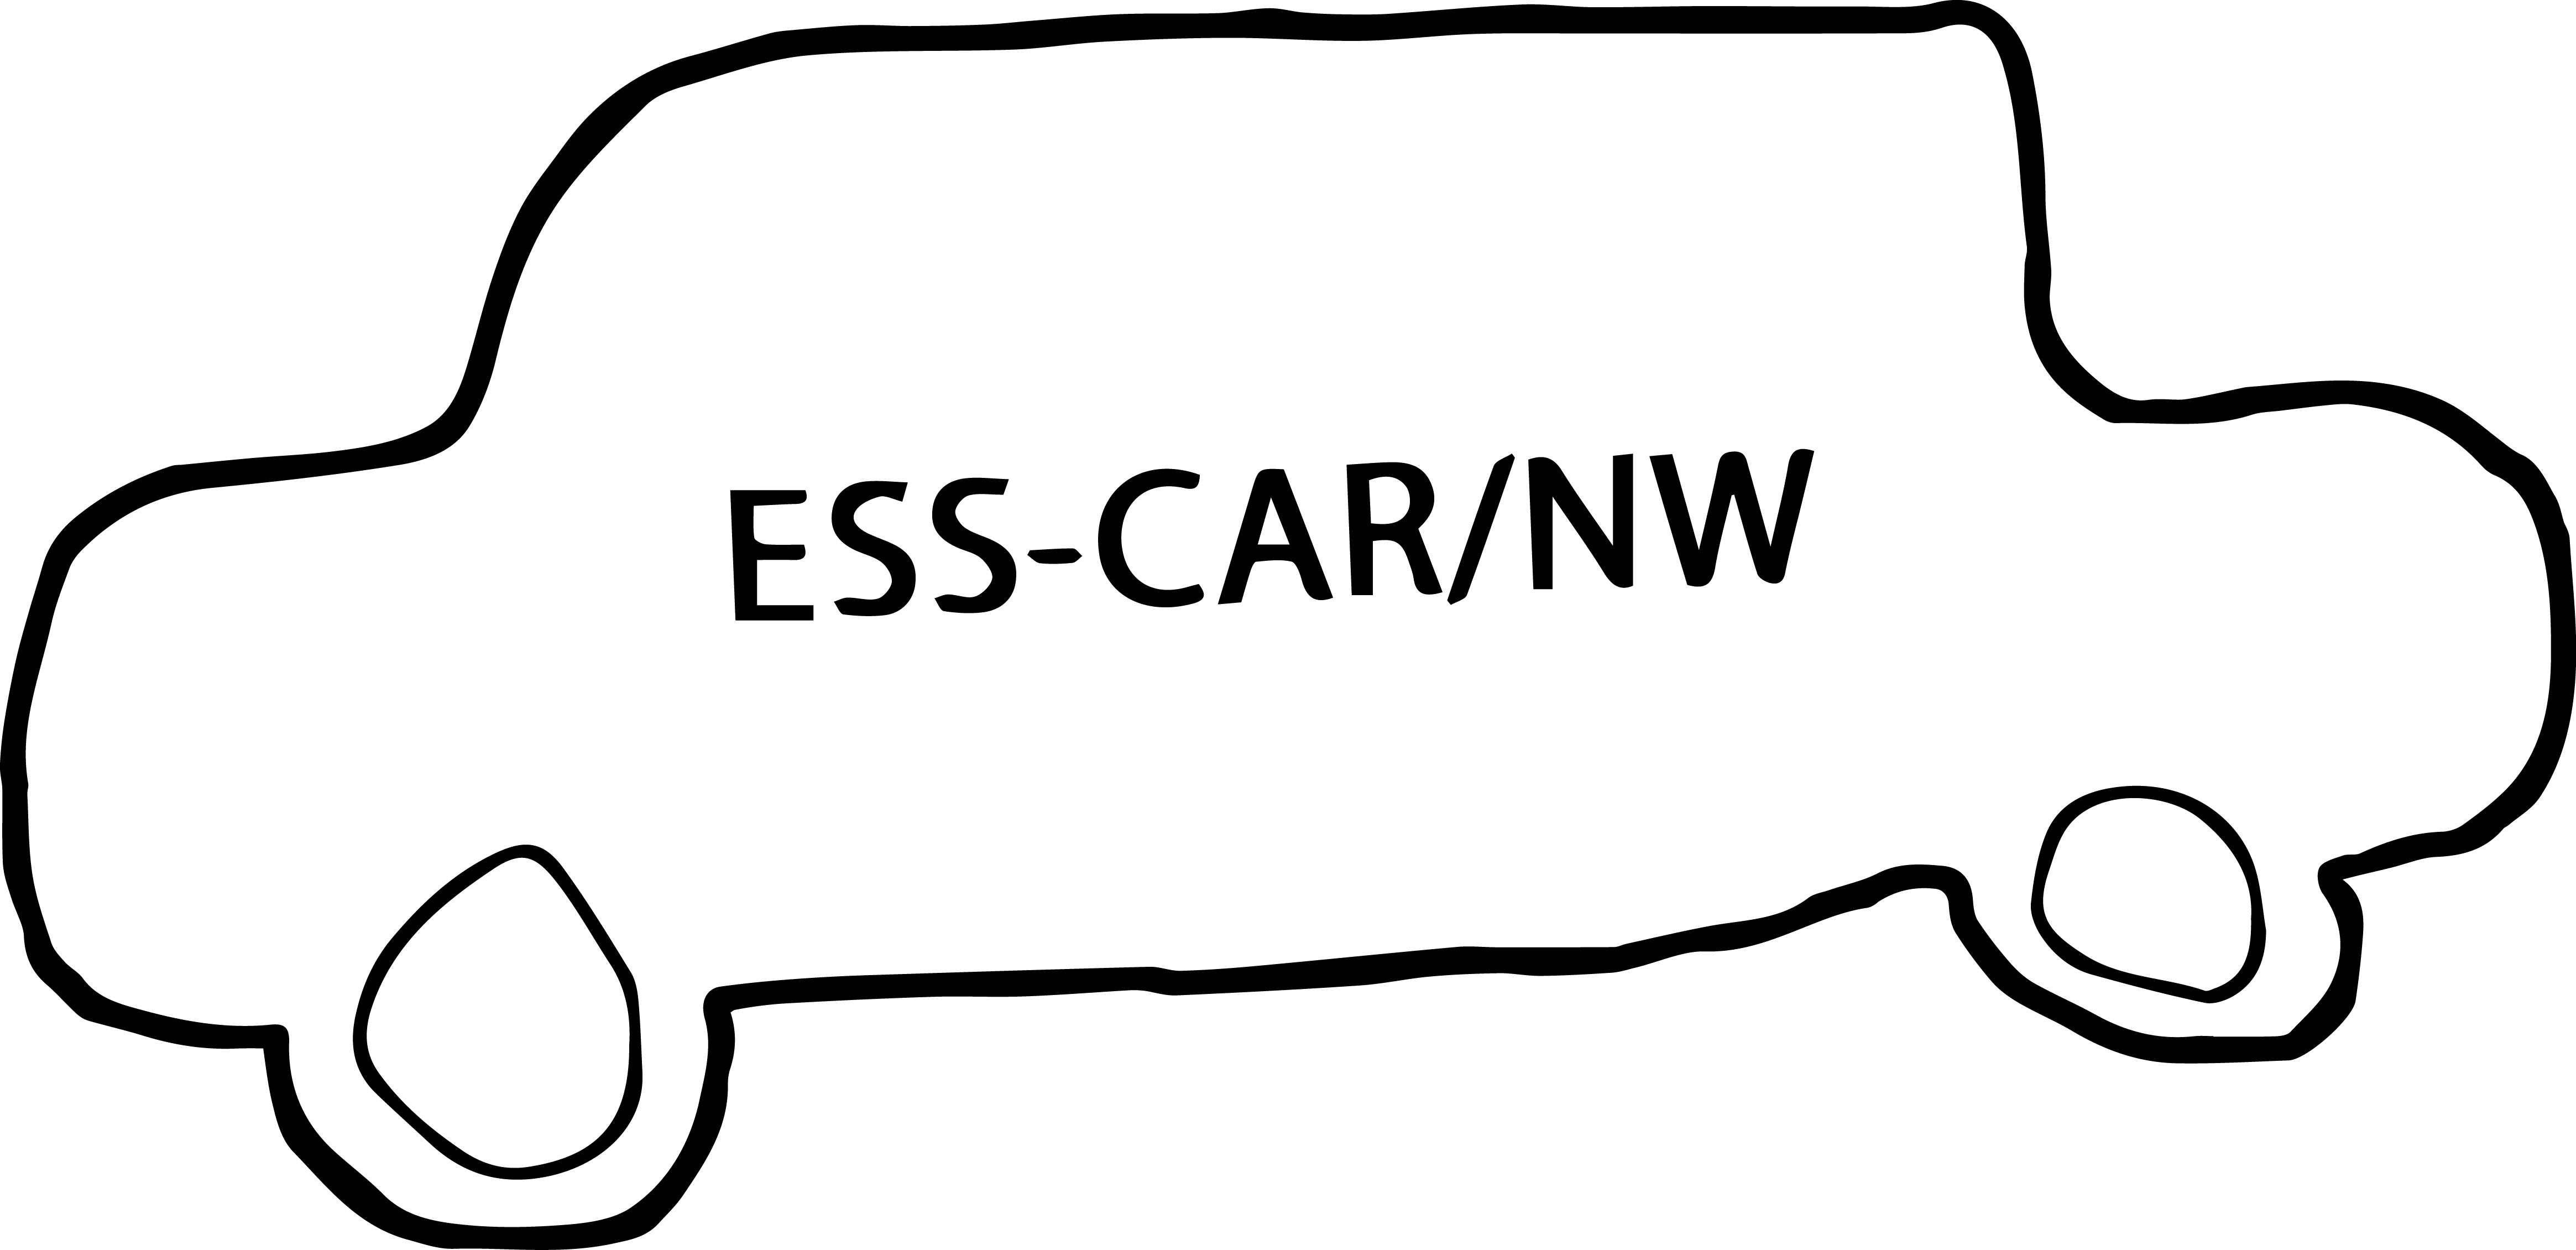
\includegraphics[scale=0.4]{funLogo.png}
	\end{figure}
	%------------------------------------------------
	%	Date
	%------------------------------------------------
	
	\vfill\vfill\vfill % Position the date 3/4 down the remaining page
	
	{\large\today} % Date, change the \today to a set date if you want
                       % to be precise
	
	%------------------------------------------------
	%	Logo
	%------------------------------------------------
	
	%\vfill\vfill
	%
\includegraphics[width=0.2\textwidth]{placeholder.jpg}\\[1cm]
        % Include a department/university logo
        % - this will require the graphicx package
	 
	%-------------------------------------------------------------------
	
	\vfill % Push the date up 1/4 of the remaining page
	
\end{titlepage}

%-------------------------------------------------------------------------

\clearpage
\section*{Abstract}
Abstract starts here,
what should be included:

The problem issue subject being addressed

How the problem is tackled

Overview of the results, and indication as to what level they solve the problem.

Implications of the results

%-------------------------------------------------------------------------
\clearpage
\tableofcontents

%-------------------------------------------------------------------------
\clearpage
\listoffigures

%-------------------------------------------------------------------------
\clearpage
\listoftables

%-------------------------------------------------------------------------
\clearpage
\section{Introduction}
This report presents the process and results of two projects "Embedded Service for Self-adaptive Network" (ESS-NW) and "Embedded Service for Self-adaptive Car" (ESS-CAR). This chapter will start by describing the background of the two projects. The next thing to be described is formulation, goals and motivation of the two projects. Following this will be a short discussion on the delimitations for our team. The last part of this chapter will present an explicit report disposition which helps readers to get a sense of the overall report.

\subsection{Background}

\subsection{Project Description}
The two projects "ESS-Car Embedded Services for Self-Adaptive Car" and "ESS-Network Embedded Services for Self-Adaptive Network" were provided by professor De-Jiu Chen at KTH Royal Institute of Technology. The idea of the two projects are from Viktor Karlquist's master thesis [??] where he presented a design and an implementation of an automotive experimental platform for ADAS. And the "ESS-Car" team from last year's MF2063 course has already implemented an autonomous vehicle prototype based on the thesis. Our projects are focused on the development and extension of the prototype.

\subsubsection{Project Goals}
The goals of the two projects could be divided into two parts, goals concerning the network implementation and goals concerning the remaining hardware and software system architecture.
The overarching goal of the network implementation part was to configure the network using software defined network method which could help researchers explore what network implementations can be beneficial in this kind of autonomous vehicle infrastructure. The overarching goal of the rest part became to increase the robustness of the system and to implement additional vision services into the system.

\subsubsection{Project Challenges}
The main challenge we faced during the process of projects was to have too many nodes in the system which greatly increased the burden of debug and test. Another challlenge was the data transfer between the local service and Vsome/Ip service in the Beaglebone. There was also a challenge coming from car assembly in which case every node shall be installed on the car and work smoothly. 

\subsubsection{Prototype formulation}
Our final prototype fulfils most project requirements we proposed at the beginning stage while there are still some requirements missing. This section will only describe what we have implemented.

The prototype is able to measure current distance and speed data and detect defined flags. All nodes are mounted on the car and connected to the network. The network consists of SDN switches and controller is support network and the other network which is made up of Beaglebones is main network. Meanwhile, eanch of Beaglebones has its seperate function, one for reading distance data and sending steering angle, one for reading speed data and sending target speed. These two Beaglebones act as SPI master in SPI communication who have two slaves each. The last Beaglebone acts as the system controller. Also a Raspberry is directly connected to the network providing object detection function. Four arduinos are used to carry out specific functions, and communicate with corresponding Beaglebone through SPI.
The prototype has two control modes, shell mode and automotive mode. In the shell mode, users could send commands from controller Beaglebone to other Beaglebones, then gather required information or change the status of the prototype. In the automotive mode, a statemachine will run which try to maintain the speed of the prototype and avoid collision. 


\subsection{Delimitations}

\subsection{Report disposition}
Chapter 1 describes the projects' background and gives an introduction to the two projects. Chapter 2 provides a short description of theories used in the projects. In chapter 3, The methods, tools and techniques used to solve the problems in the project are specified. The implementation of the autonomous vehicle prototype is presented in chapter 4. Chapter 5 describes how we verify and validate the prototype. The results of the two projects are shown in chapter 6, then chapter 7, has a discussion and a conclusion on the final results. The last chapter, chapter 8, lists some future work.  
%-------------------------------------------------------------------------
\clearpage
\section{Literature Review and State of the Art}

\subsection{Network}
%-------------------------------------------------------------------------
\subsection{Software defined network}
Software-defined network (SDN) is a type of network where a controller decides how the traffic in the network should go. In a traditional network is the intelligence in the switches and they decided on what port the package should be sent out on. In SDN is a device called controller connected to all switches and monitors the traffic load on the links and find the most optimal path between node A to node B. The controller’s task is to request information from the switches about what links are up or down and the traffic load with this information and decides how packages should be forwarded on the switch. Because the controller can monitor the topology of the network is it easy to scale the network with new nodes and switches\cite{doi:10.1002/sec.1737}. 


%-------------------------------------------------------------------------
\subsection{Serial Peripheral Interface}
Serial Peripheral Interface (SPI) is a synchronous serial interface specification for short distance communication. SPI supports full duplex mode using a master-slave architecture with one single master, and the SPI master originates the whole communication. The SPI bus has four logic signals: serial clock (SCK), master output slave input (MOSI), master input and slave output (MISO), slave select (SS). The detailed pin mapping of SPI master and slaves is shown in figure ??.

% figure: one master and multiple slave connection
\begin{figure}[H]
	\centering
   	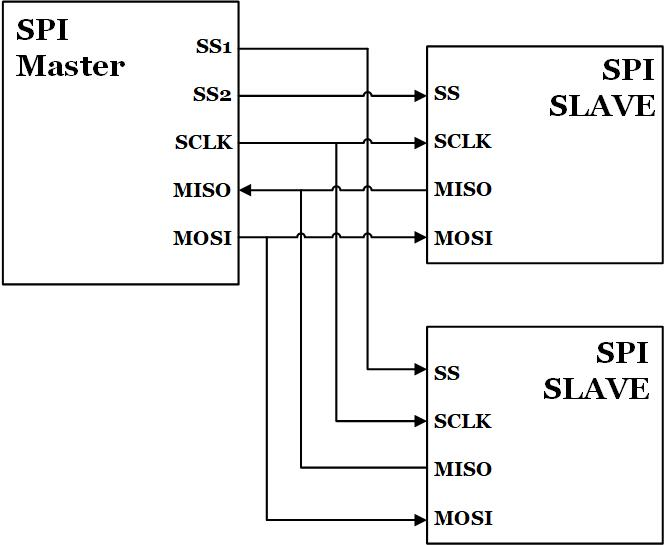
\includegraphics[scale=0.5]{spi-literature.jpg}
   	\caption{Connection of one SPI master and two SPI slaves}
    \label{fig:spi-literature}
\end{figure}

SPI has a higher throughput than those traditional transaction protocols, e.g. $I^{2}$C, UART, as it is not limited to any maximum clock speed enabling potentially high speed. And the hardware interface is pretty simple where slaves only use master's clock and are able to share the other three signals but the SS. Meanwhile, the software is not hard to implementation. For the opposite side, SPI has its limitations. There is no slave acknowledgement or hand-shaking mechanism in SPI, so the master could keep sending data to nowhere and not know it.

\subsection{SOME/IP}


%-------------------------------------------------------------------------
\subsection{Assembly of the car}
To make the car moving all the devices and components on the car has to placed on the car and because of there many devices on the car that communicates via SDN and has all of them be placed in an efficient way. To do that needs some kind of platform to be created to mount all the devices on and they are close to the other devices its depended on. 

%-------------------------------------------------------------------------

\subsection{Power Supply}
The car uses a 2 cell lithium battery what delivers a voltage of 7.2V. On the car is two different voltage level used, the first one is at 9V for a switch, and the second level is at 5V to power all the other components. 

To generate a voltage at 9V from 5V or 7.2V has some kind of DC-DC converter be build to generate a higher voltage. 


%-------------------------------------------------------------------------
\clearpage
\section{Methodology}
%%%%%%%%%%%%%%%%%%%%%%%%%%%%%%%%%%%%%%%%%%%%%%%%%%
%TODO chapter overview
%-------------------------------------------------------------------------
\subsection{Software defined network}

The SDN switches used in this implementation is the Zodiac FX from Northbound Networks. They are switches made to support OpenFlow protocol and is designed to be used in SDN networks. On the switch is 4 ports there one port that has to be connected to the controller, all the other ports can be used to connect devices on. As shown in figure ?? is 5 devices connected to the network and the switches has to be connected to each other has the network 3 switches. 

Mininet is a Python-based application what an SDN network topology can be created and simulated to test that the controller works and analyse how the network will operate. The program also has the opportunity to connect the simulated topology to your physical SDN controller. 

The car network topology was simulated in Mininet to analyse its behaviour, and to develop code for the controller. Under this test did we discover what that Mininet simulation had a much lower delay then the real implementation had, even then the extra settings on the links and nodes were added. This resulted that Mininet could not be used to analyse the best topology for the car. It was instead used to simulate the network to create a code for the Ryu controller. To analyse the Car network was two different Mininet scripts created, one was to use the physical raspberry pi controller and the second one was to use the internal version of Ryu in the Mininet VM. For the external simulation to work has the script be configured with the right ip-address to the raspberry pi. 

\subsection{Software Architecture}
The driving system consists of several layers of software and communication. Figure~\ref{fig:bbb_arch}
and~\ref{fig:rpi_arch} give a broad overview of how the software is structured. A custom driving software
is running on the client BeagleBone. This can be either an interactive shell or a test suite
of commands for testing and debugging basic functionality or a more intelligent autonomous driving
software. The custom driving software controls the car through a library called ESSPrototype.

ESSPrototype is a C++ library that represent fundamental functionality for maneuvering and monitoring
the car. Some examples include controlling the steering, getting speedometer readings and checking if
the distance sensors are online. Input and output to ESSPrototype is done via a UNIX shared memory and
the IO packets can be seen in Figure~\ref{fig:packets}. Table~\ref{tab:packets} contain brief
descriptions of the packets.

At the other end of the UNIX shared memory that ESSPrototype uses, a client/server software
runs and it is based on an application-layer protocol called SOME/IP \cite{someip}. The C++ implementation of the 
protocol used for this project is VSOMEIP \cite{vsomeip}. 


\begin{figure}[H]
	\centering
   	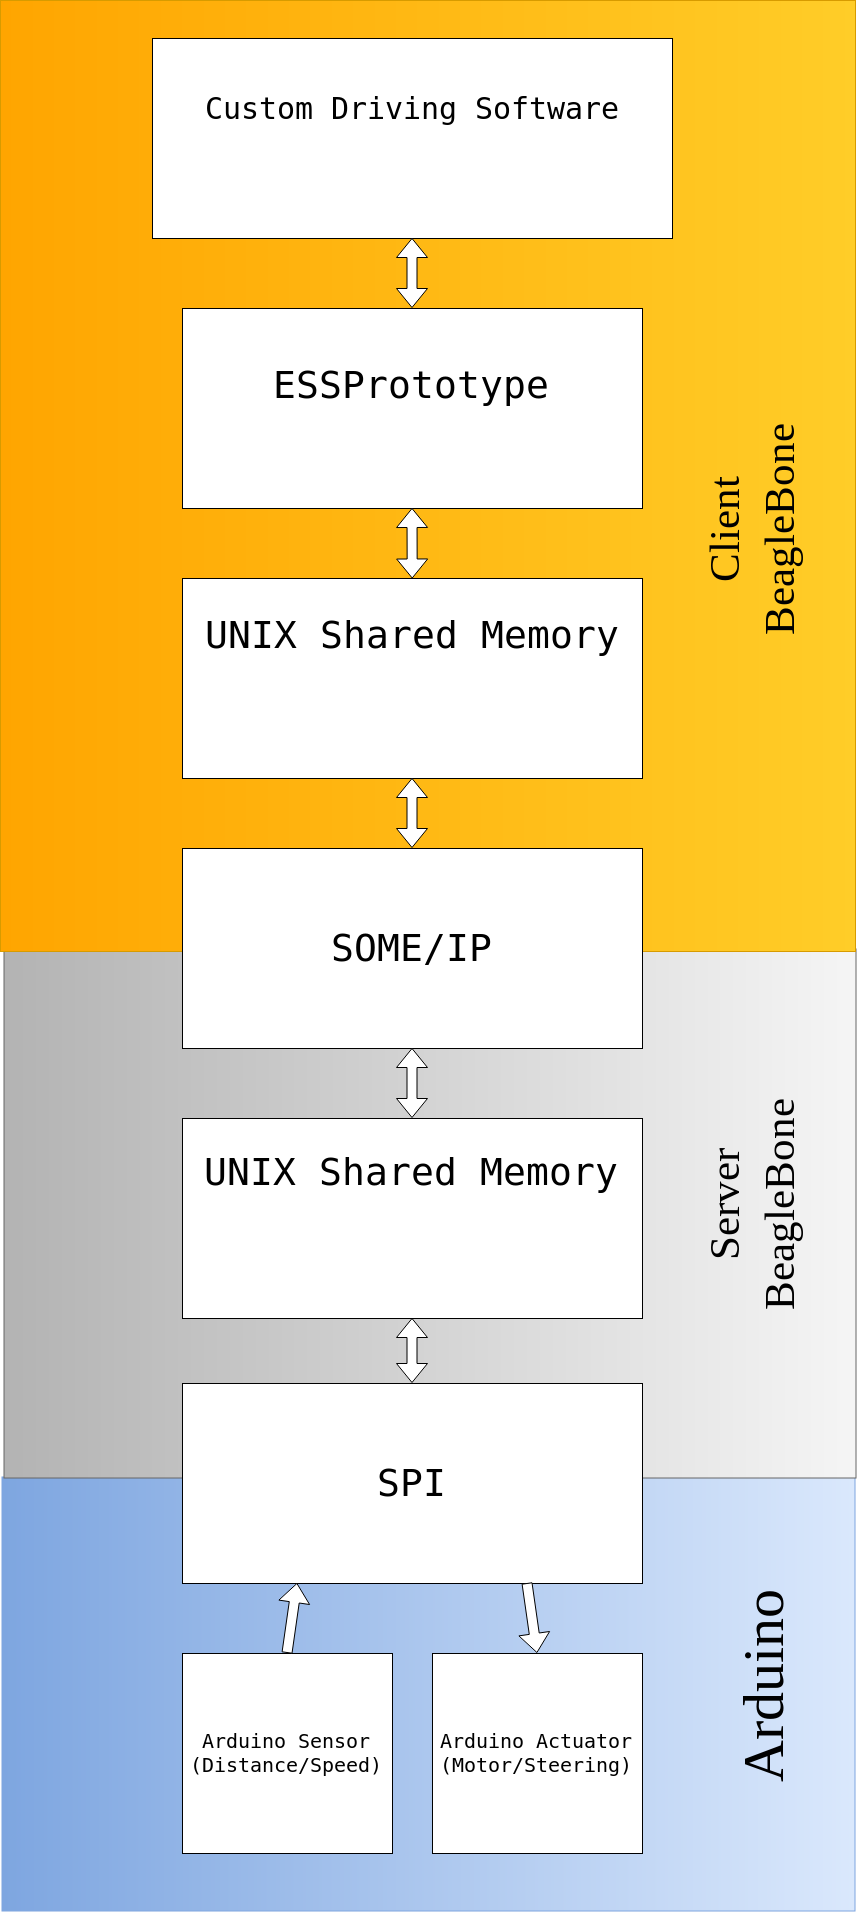
\includegraphics[scale=0.25]{arch_bbb.png}
   	\caption{Overview of how the service beaglebones are part of the software architecture.}
    \label{fig:bbb_arch}
\end{figure}

\begin{figure}[H]
	\centering
   	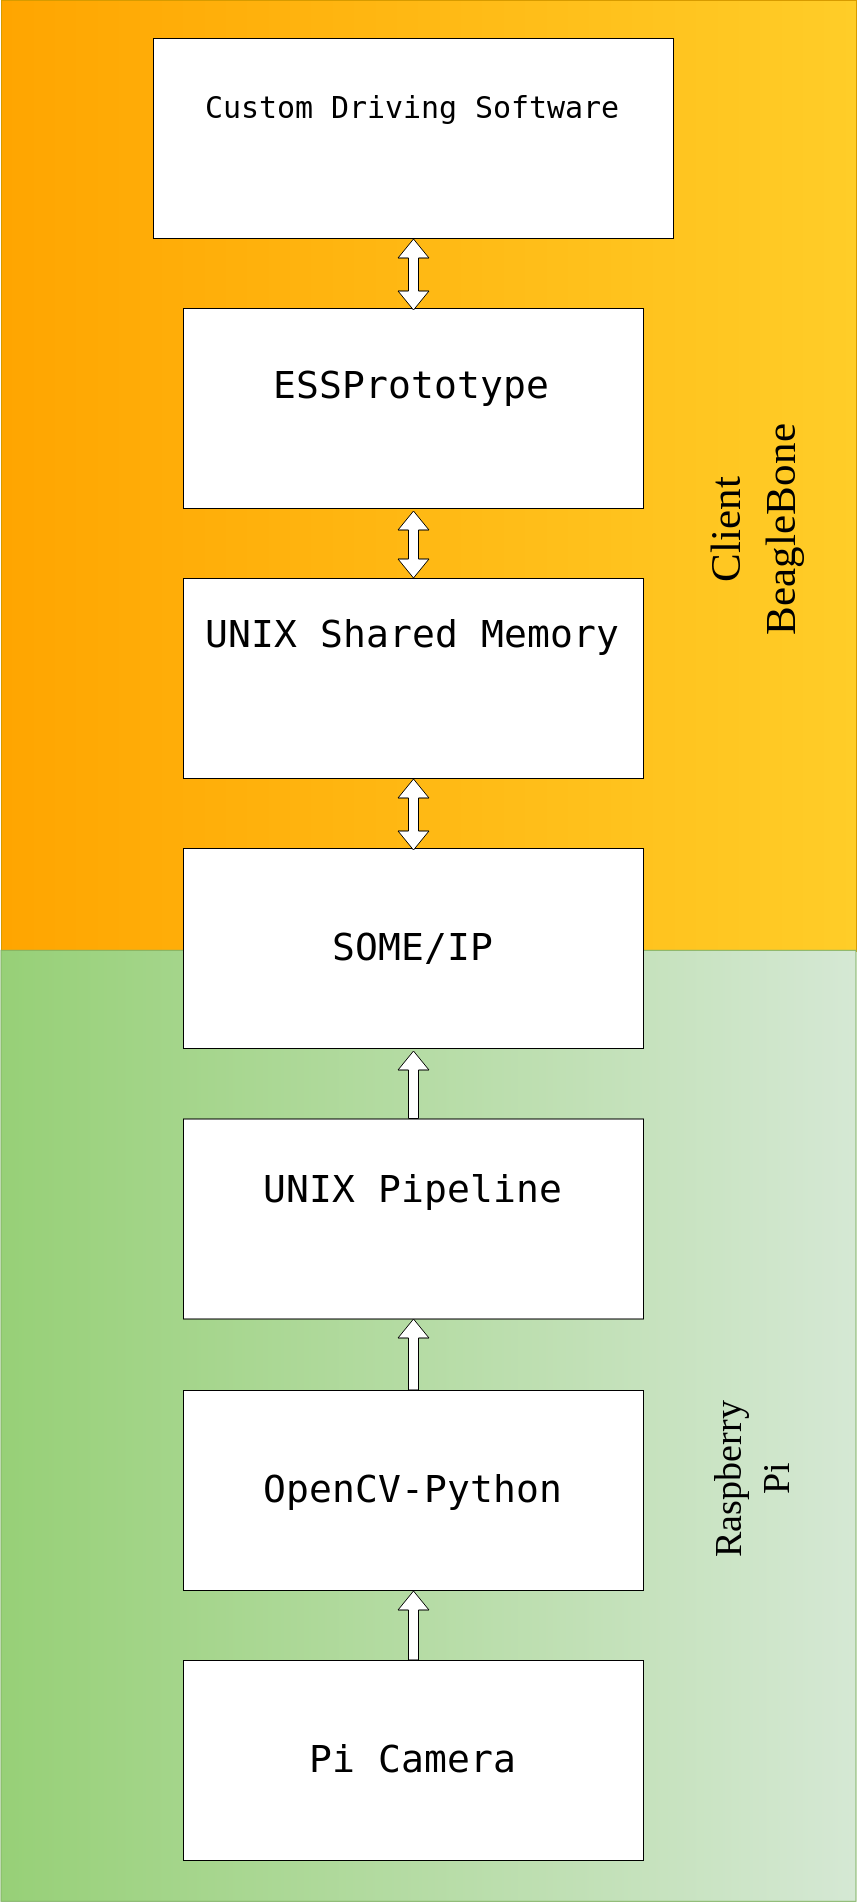
\includegraphics[scale=0.25]{arch_rpi.png}
   	\caption{Overview of how the camera service Raspberry Pi is part of the software architecture.}
    \label{fig:rpi_arch}
\end{figure}

\begin{figure}[H]
	\centering
   	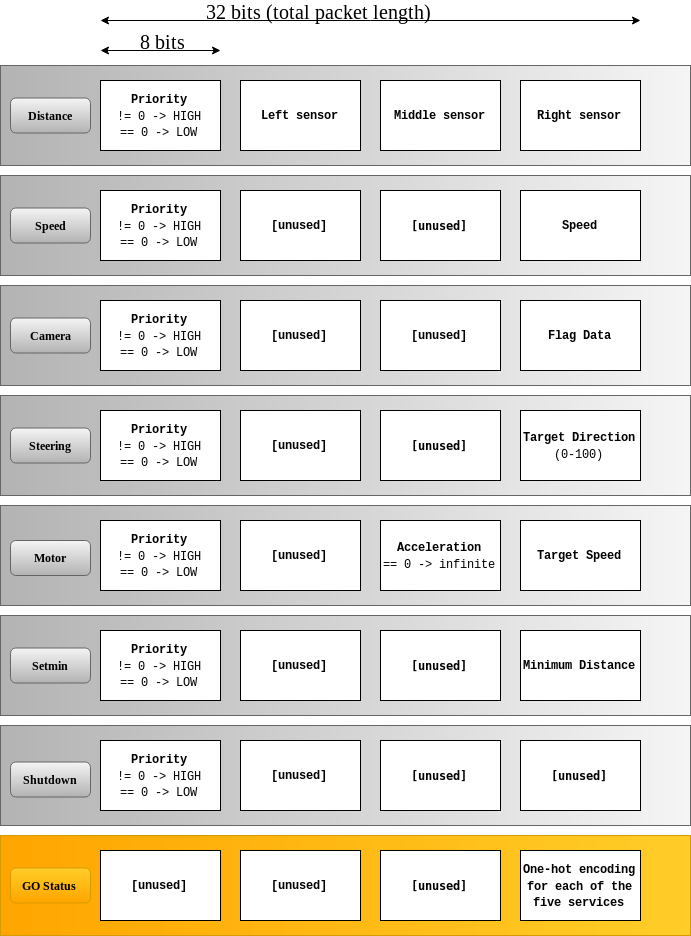
\includegraphics[scale=0.5]{packets.png}
   	\caption{Input/Output packets handled by the ESSPrototype library.}
    \label{fig:packets}
\end{figure}

\begin{table}
  \caption{Brief descriptions of the packets handled by the ESSPrototype library.}
  \label{tab:packets}
  \centering
  \begin{tabular}{|l|l|} \hline
    \textbf{Type} & \textbf{Description}  \\ \hline
    Distance & Measurements from the distance sensors (in cm) \\ \hline
    Speed & Measurement from the speedometer (in cm/s) \\ \hline
    Camera & Feature extraction from the camera containing color and position information  \\ \hline
    Steering & Desired steering angle (0 means full left, 100 means full right)  \\ \hline
    Motor & Desired speed along with the acceleration for achieving that speed \\ \hline
    Setmin & Set threshold value for when the motor should perform an emergency break  \\ \hline
    Shutdown & Packet that shuts down all services on a node, no data payload required  \\ \hline
    Go Status & Packet that shows what services are available (distance, speed, camera, motor, steering)  \\ \hline
     \end{tabular}
\end{table}

%-------------------------------------------------------------------------
\subsection{VSOME/IP}

%-------------------------------------------------------------------------

\subsection{Project management}
Scrum project management is used during the process of our projects.
The scrum framework has been adopted for use in this process because of it being agile as well as the fact that most group members had some type of previous experience or knowledge with it. Both software and physical tools were used for monitoring the projects progression. Excel was for example used to keep track of milestones, earned value and the resource plan and the online tool trello was used alongside a physical whiteboard to keep track of scrum sprints and the project backlog as depicted in figure \ref{fig:scrum-board}. A lot of design was also produced and kept on whiteboards as to promote discussion within the group and to keep everyone updated with updates or changes to design or models.

As with all projects where the team members have no previous experience in working with eachother there will be a roll-seeking phase where the dynamic of the group is slowly figured out and which different positions the team members fit in. To make the group get into the process of working quickly the group deceided to follow the results given by the belin test which was performed by all group members.

Setting up clear milestones for the project was very benificial in managemnt as it helped to divide the project into different phases in time with each ones having clear expected outcomes. This helped the project stay on track with regards to time as it could easily be followed what needed to be done and when.

To ensure smooth progress it was deceided to have weekly meetings with the stakeholders were all group members could go through what they had done the previous week and receive feedback from the stakeholders. The feedback could be general tips and aid on the current assignment or that they wanted to steer a part of the project in a different direction or note that there might have been some part or parts that have been overlooked in the design or implementation. These meetings were also usefull for rasising issues that were encountered during the development with our project sponsors. The messaging app called Slack which is often used by development teams in industry was also used by the project group including the sponsors. This allowed the group to bring up urgent issues with the project sponsors directly, without having to wait until the next weekly meeting, and getting a quick response as soon as possible.


\begin{figure}[]
	\centering
   	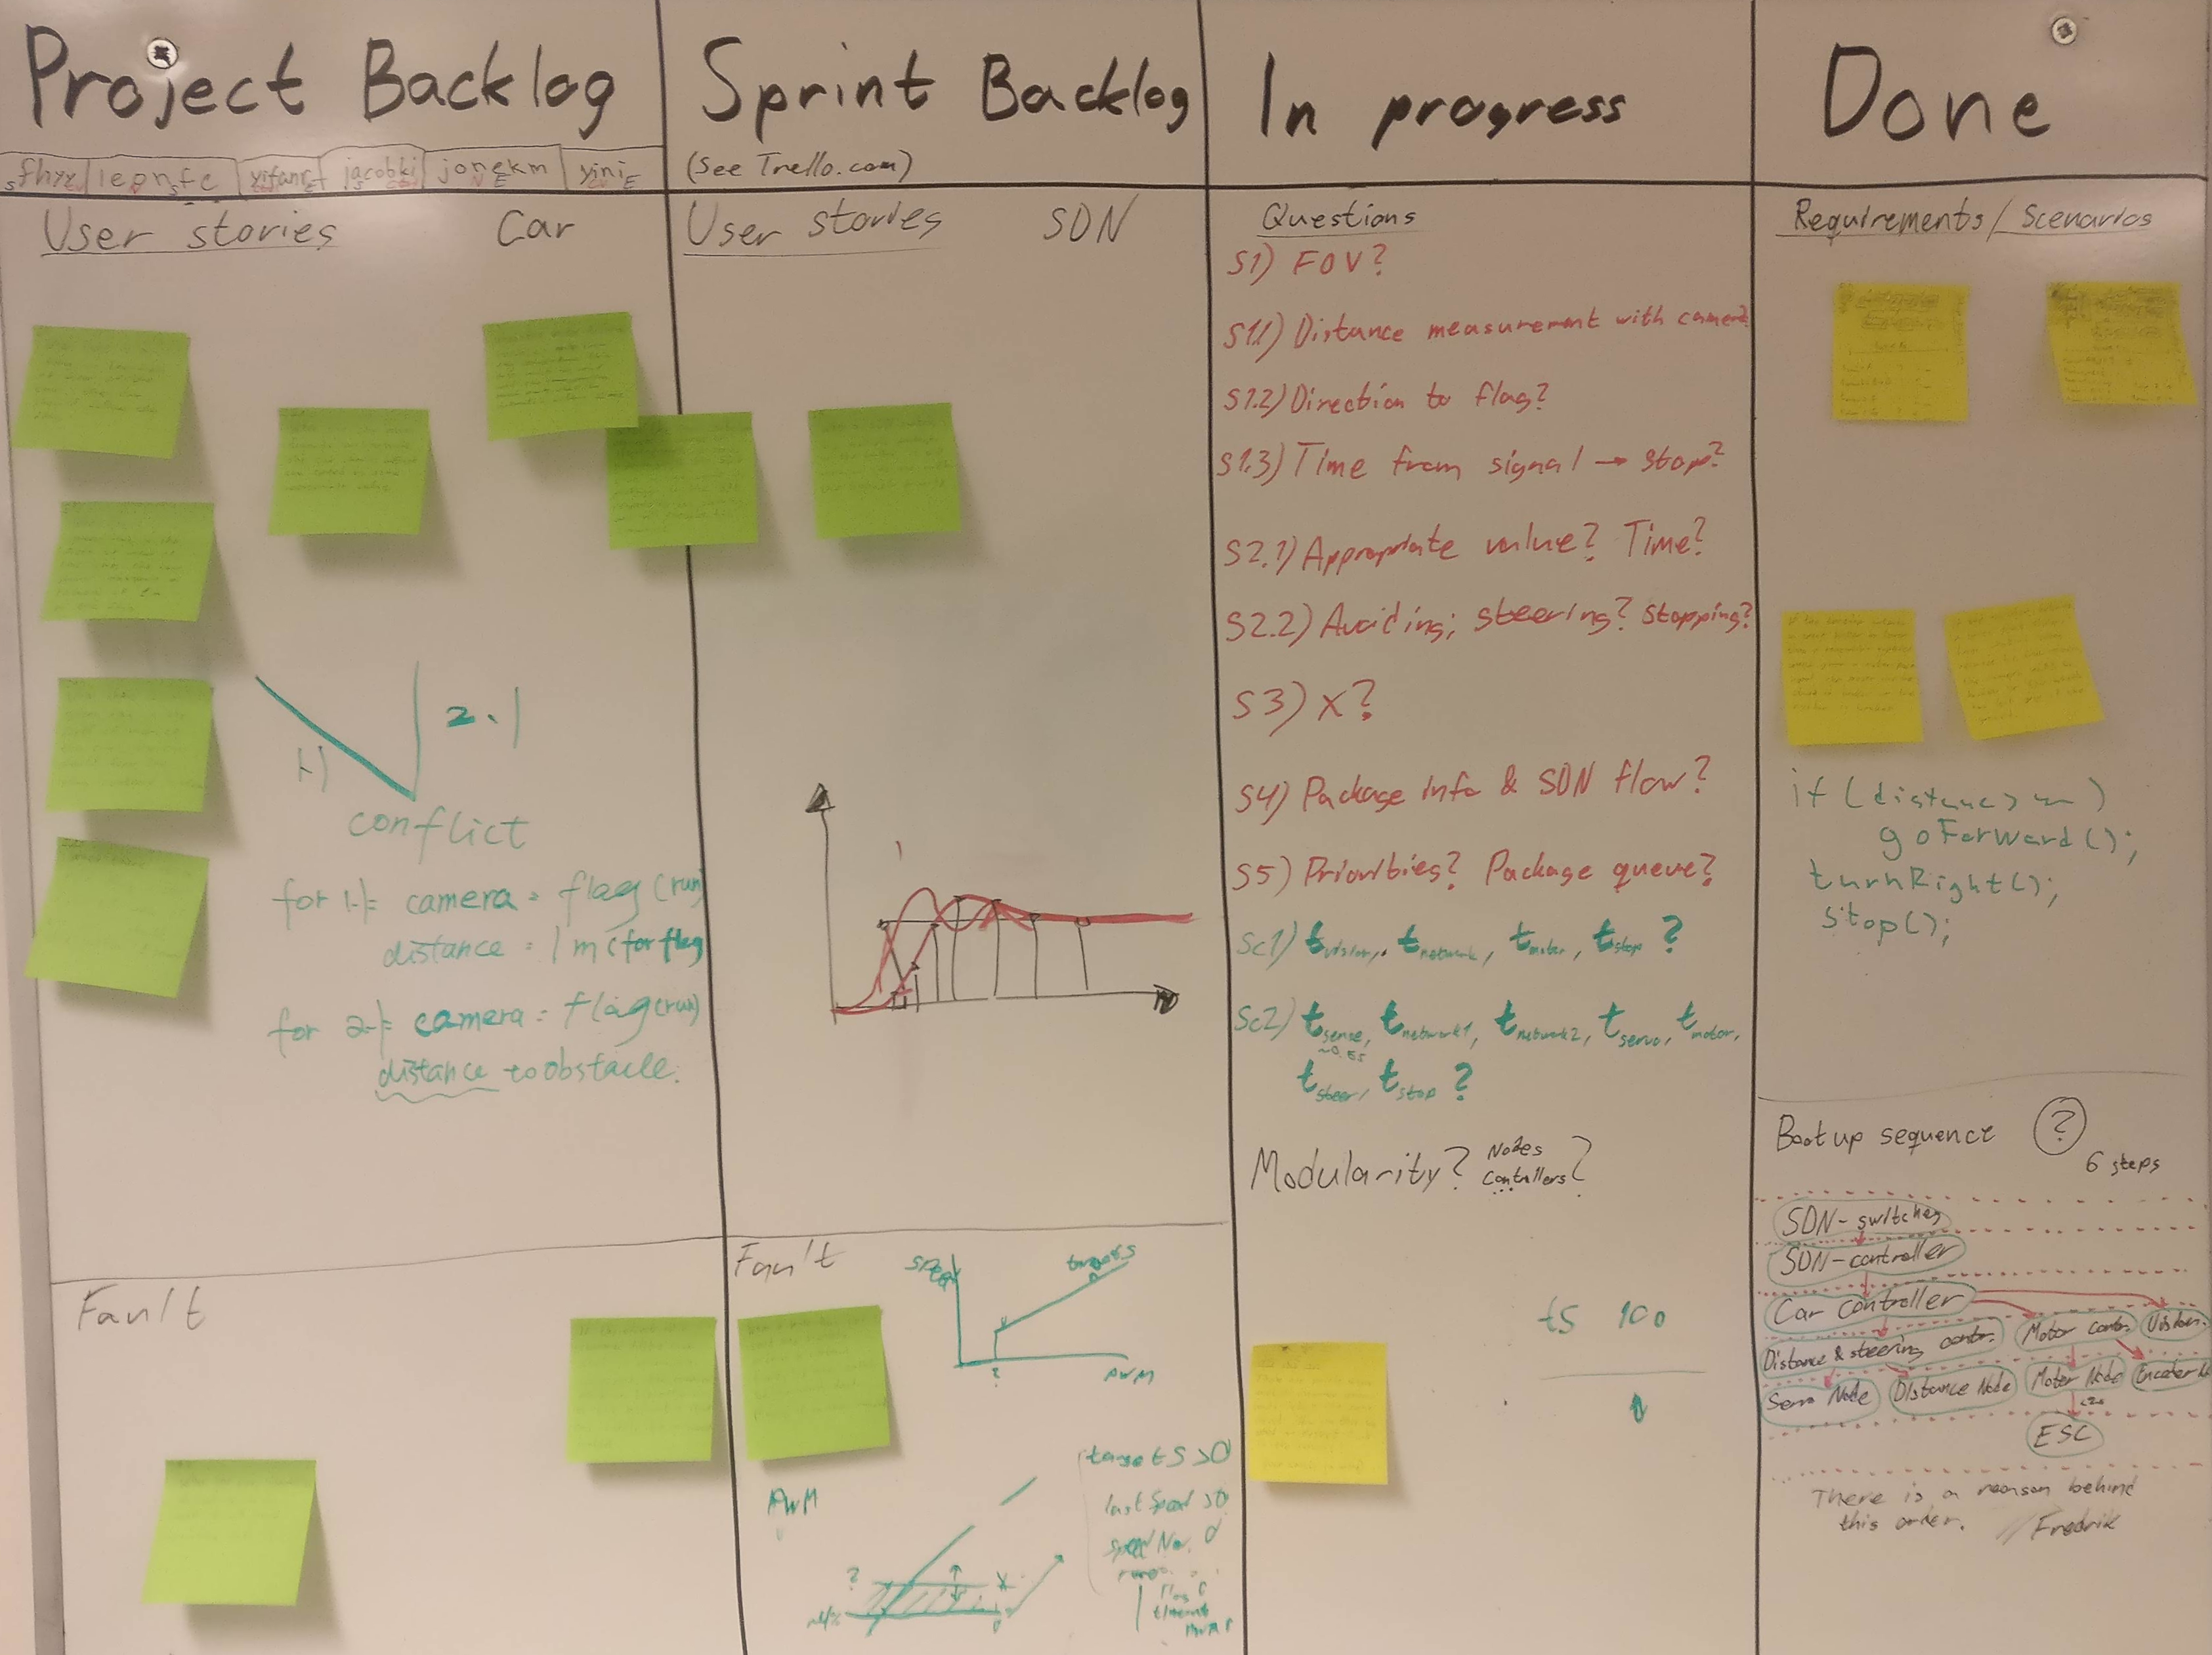
\includegraphics[scale=0.5]{scrum-board.jpg}
   	\caption{Scrum board continously used throughout the project}
    \label{fig:scrum-board}
\end{figure}

% informal leadership (good group dynamic required less leadership)


%-------------------------------------------------------------------------
\subsection{Assembly of the car}

The car platform used in this project is a car platform is Turnigy SCT 2WD 1/10 Brushless Short Course Truck (KIT) upgraded version and it was provided by the stakeholders at the start of the project. 

To place all the required components on the car had some kind of platform be created to mount everything on. The requirements for the platform is if passible the car chassis should be able to fit on top of the car, all the device should be mounted on it and it should be easy to remove from the car. 

To make this platform was it first draw in a Cad Fusion 360 to make a 3D model of the car. This model could then be used to add models of the devices used in the car to find the optimal place for them, so the are places in at an easy position to get access too and close to its devices its depended on. The result of the design is shown in figure \ref{fig:3d_platform}. 

\begin{figure}
	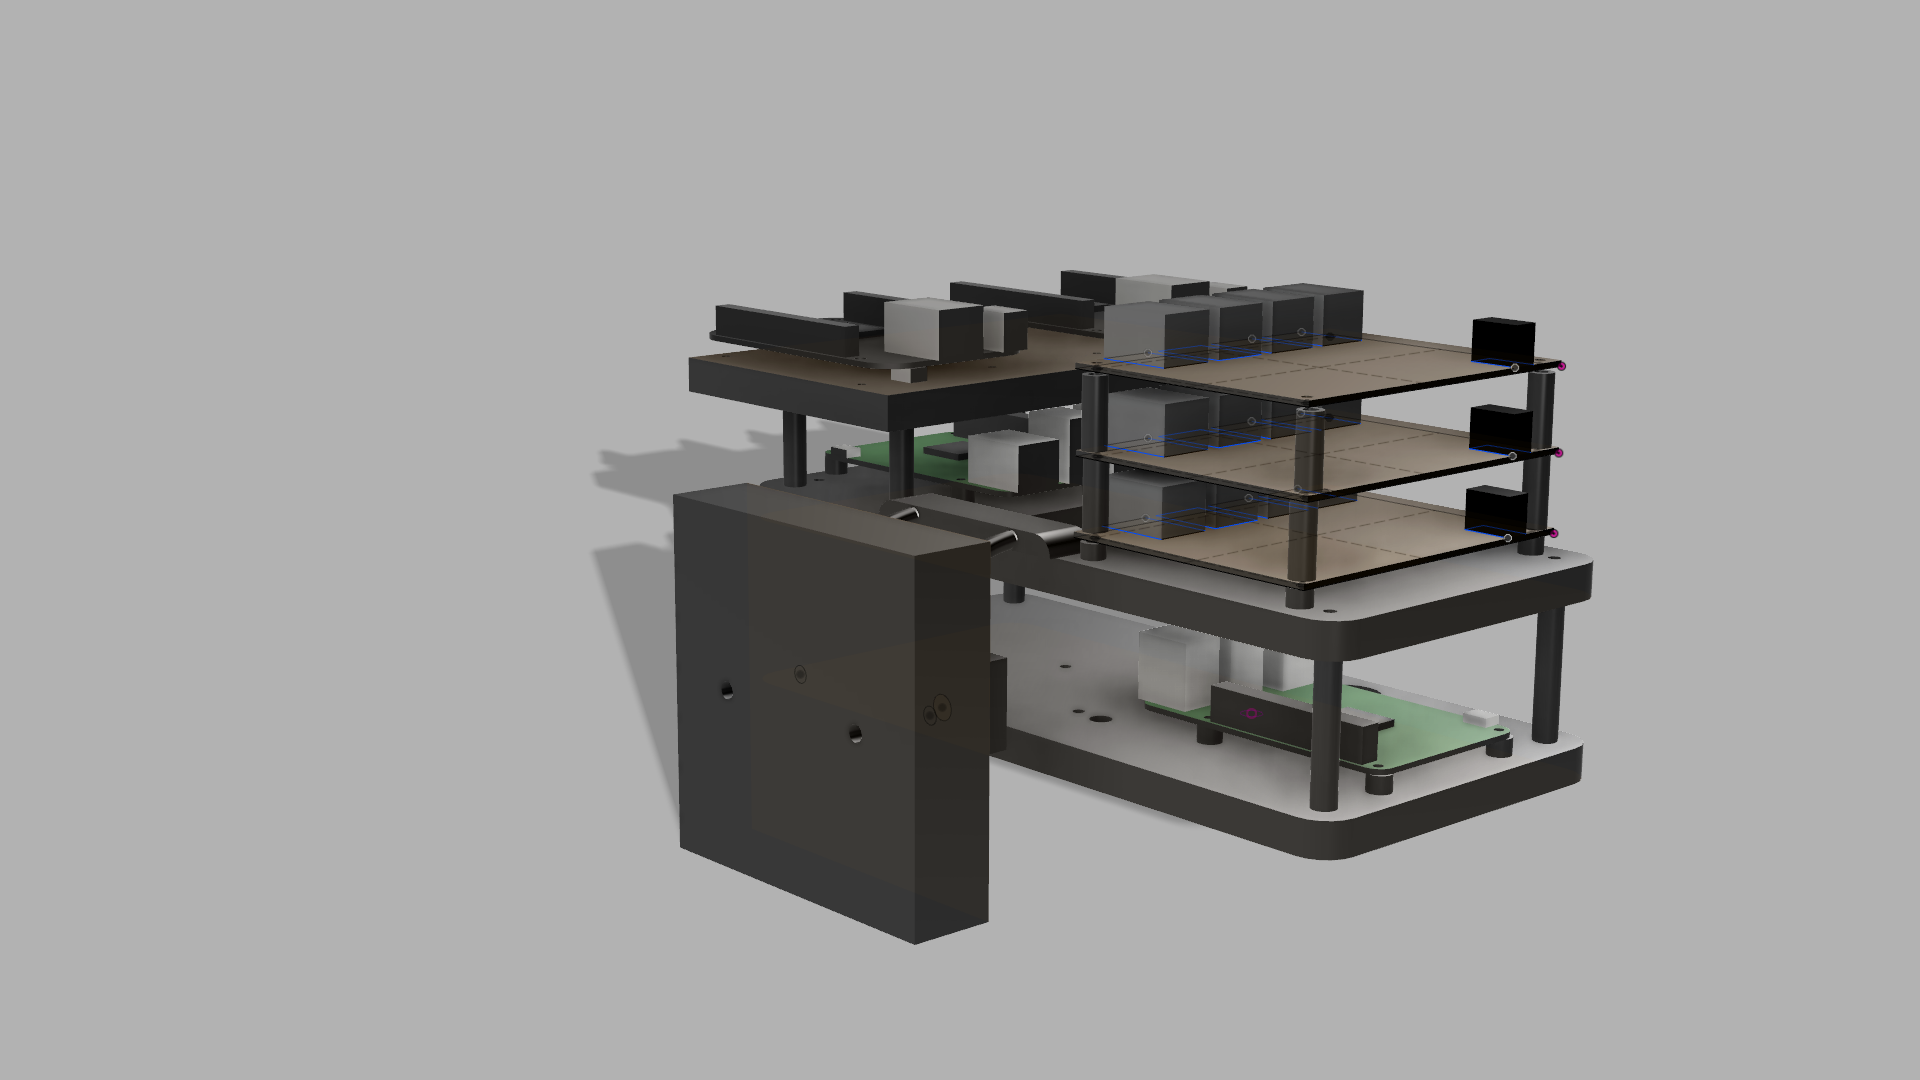
\includegraphics{platform.png}
	\caption{3D model of the platform}
	\label{fig:3d_platform}
\end{figure}

%-------------------------------------------------------------------------
\subsection{Power Supply and PCB}

The power supply for the devices on the car is done via two different levels one at 5V and the second one at 9V. This requires some converter to converts the 7.2V from the battery to 5V and 9v. The 5V DC-DC converter is a Turnigy USBEC-15A it as voltage regulator made especially for lithium batteries and has input voltage range between 6V-12.6V and it can deliver 5V volt as output. This converter was used because it was already provided in the material we received from the stockholders and because it indicates how much power there is left in the battery. The most important reason the converter module was used is because lithium batteries are sensitive can easily be damaged, so it was a smaller risk the battery would be damaged and affect the project development. 

The second converter is to generate the 9V and this is done via a DC-DC converter called boost converter. The idea of the boost converter was it should be connected after the first converter and would have an input voltage at 5V to generate a 9V output and a current of 0.6A. The reason it uses the 5V voltage level as input and not the 7.2V from the battery is to have all the powering done via the Turing converter and would not have something connected to the battery, that could damage it. The design for the boost converter was done in a program called MPLAB Mindi and is an analogue simulation program from Microchip, and it was used because the IC chip MIC2253 is from Microchip and it was provided as a PSpice simulation component so the circuit could be analysed. The MIC2253 is DC-DC boost converter wat has a switching frequency of 1MHz has an input voltage range between 2.5V-10V. The schematic for the boost converter is shown in figure \ref{fig:circuit_boost_converter} and designed form the recommendation provided in the datasheet for the MIC2253. The MIC2253 has the functionality of an Overvoltage Protection pin that is used to shit down the switch if the pin has a voltage higher then 5.6V, to solve this was to resistors R5 and R6 in parallel added to the OVP pin as shown in figure \ref{fig:circuit_boost_converter}. The values of R5 and R6 is calculated from formula \ref{eq:ovp}. To get the correct output voltage had R1 and R2 in figure \ref{fig:circuit_boost_converter} be changed to correct values. They are calculated from formula \ref{eq:vout} and the V\textsubscript{out} was set to 9V. This circuit was then simulated in MPLAB and it showed that the circuit should give an output voltage at 9V and a current peak of 0.9A, as shown in figure \ref{fig:graph_boost}. 

\begin{equation}
	9V < 1.245 * \frac{67k \Omega * (R5 + R6) }{15k \Omega * R6}	
	\label{eq:ovp} 	
\end{equation}

\begin{equation}
	V_{out} = V_{ref} * (\frac{R1}{R2} + 1)
	\label{eq:vout}
\end{equation}



\begin{figure}
	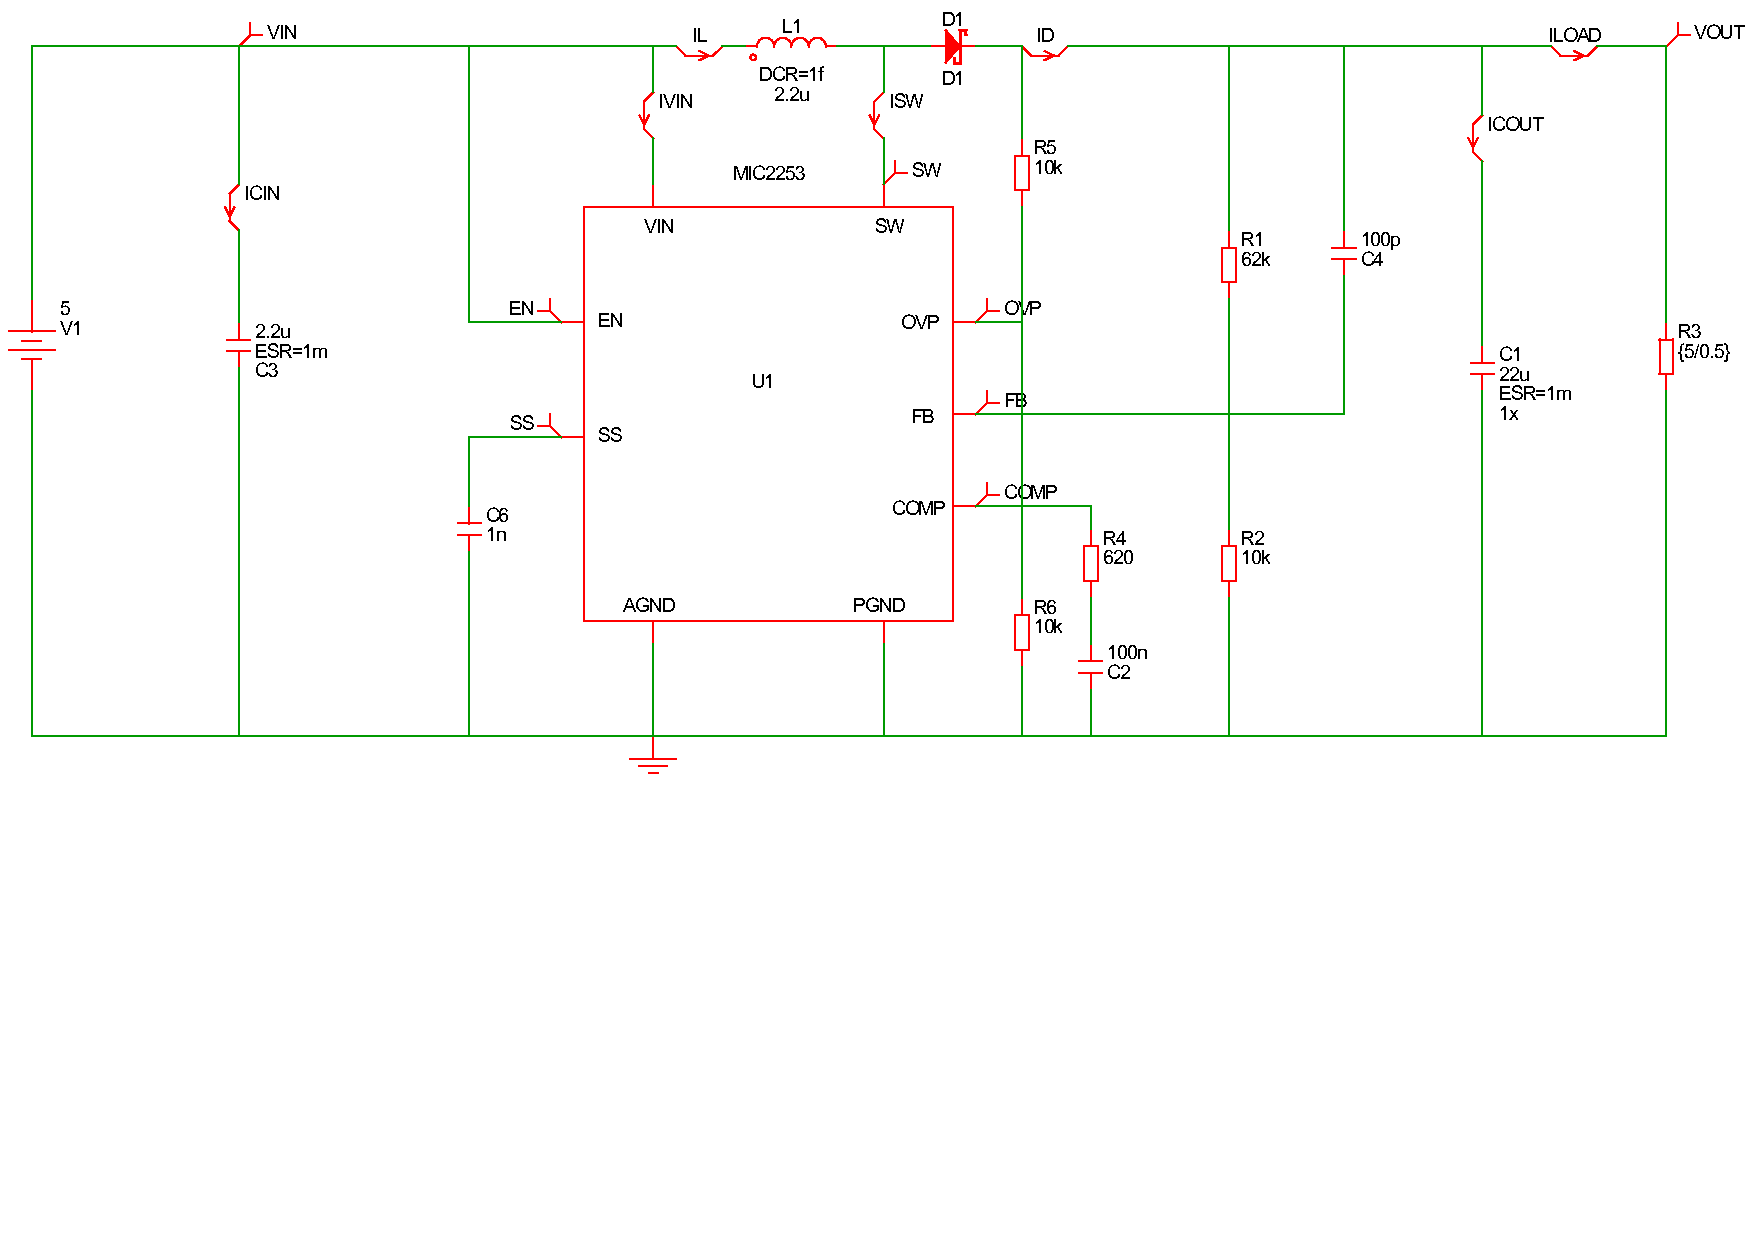
\includegraphics[width=0.9\textwidth]{boost_converter_curcuit.pdf}
	\caption{Circuit of the boost converter}
	\label{fig:circuit_boost_converter}
\end{figure}

\begin{figure}
	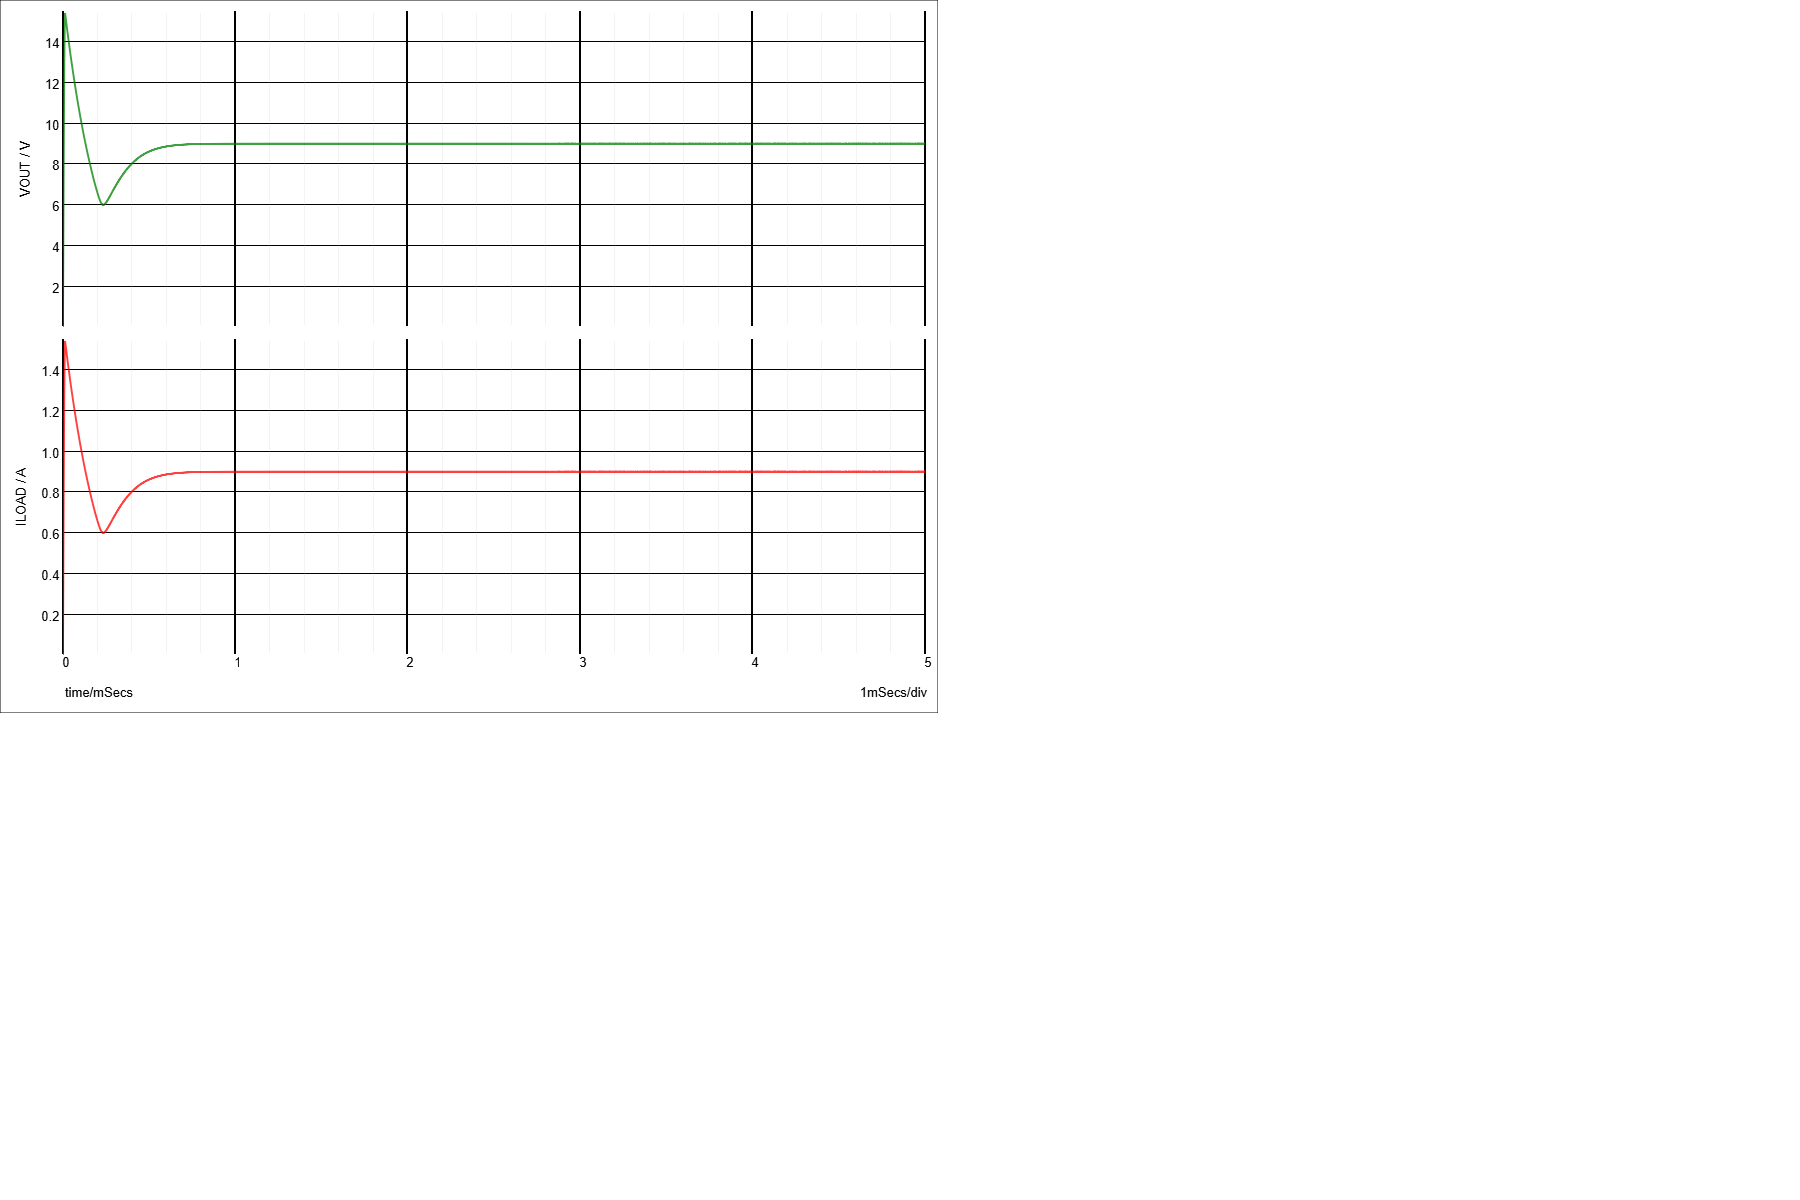
\includegraphics{graph_of_boost_out.png}
	\caption{Out puth grapth of the Boost converter}
	\label{fig:graph_boost}
\end{figure}

All the powering of the car's devices should be handled by one PCB board, that contained USB ports and the boost converter to power the external switch. There the USB-A type ports should be used to power the Arduinos, Beaglebones, Raspberry Pi and Zodiac FX. For the powering of the external switch should a cable be connected from the PCB to the switch, it also to power outlets to power the PCB board for the Arduinos. This PCB board was designed in Eagle and the result is shown in figure \ref{fig:power_pcb_layout}. 

\begin{figure}
	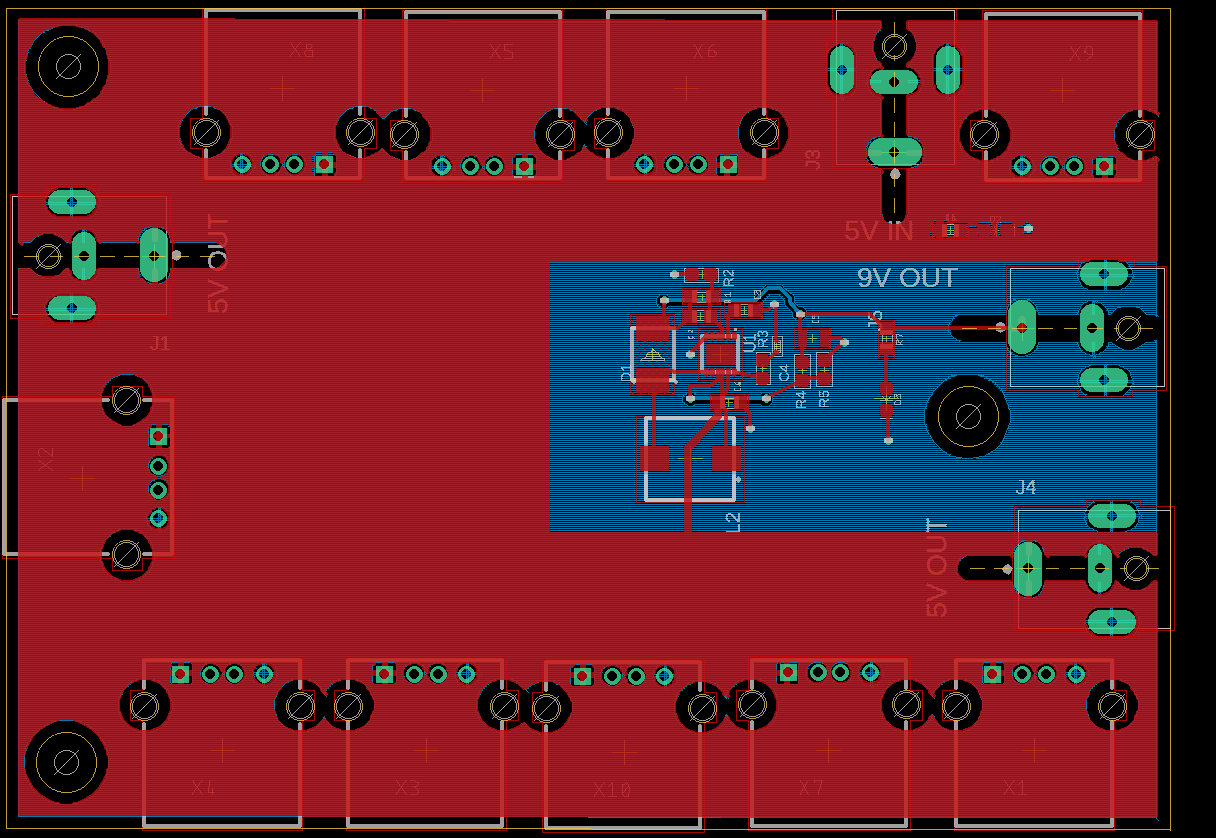
\includegraphics[width=0.3\textwidth]{power_board_layout.png}
	\label{fig:power_pcb_layout}
	\caption{Layout of Power PCB board}
\end{figure}

For the Arduinos was two PCB boards made to easily connect the SPI connection between the Beaglebones and the Arduinos, and to connect external sensors. The first board was designed to easily connect the ultrasonic sensors and the steering servo with correct Arduino. The schematic and layout of this board was also made in Eagle and is shown in figure \ref{fig:board_layout_ultra_servo}. The board is powered via a power via the DC power jack, to supply the Arduinos. On the top of the board is three connectors and they are for the Ultrasonic to be connected, and in the bottom is the connector for the steering servo. In the middle of the board is the connection to add the Logic level converter and the pins to connect the connection from the Beaglebone. 

\begin{figure}
	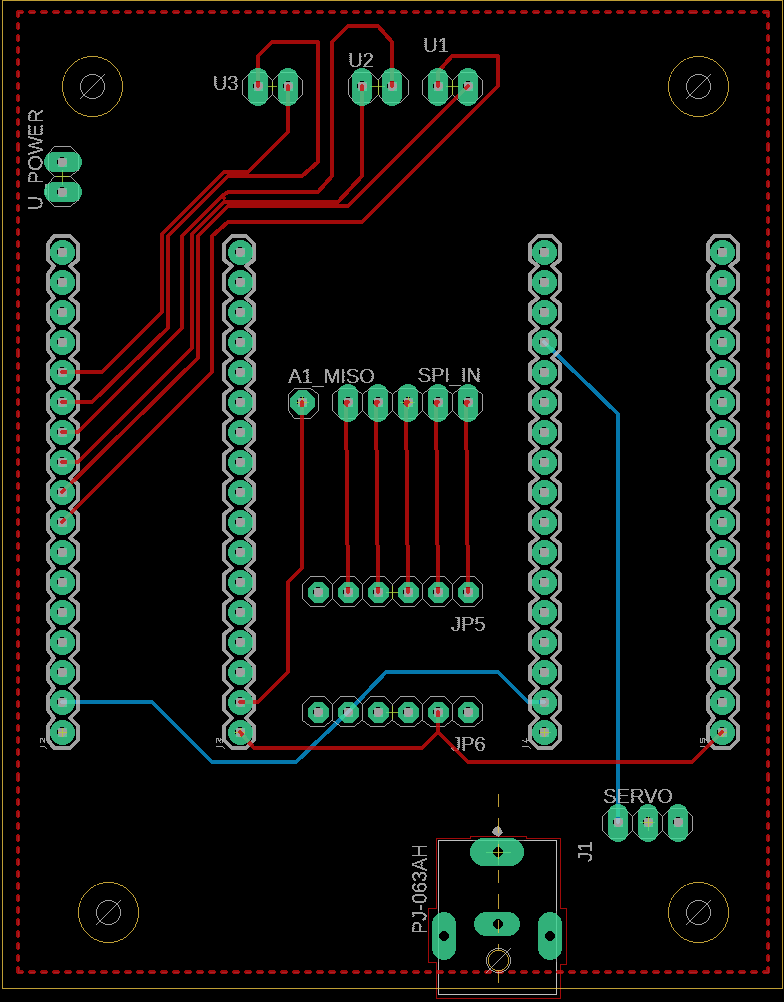
\includegraphics[width=0.3\textwidth]{borad_layout_seervo_ultra.png}
	\caption{Layout of the Board for ultrasound and steering servo}
	\label{fig:board_layout_ultra_servo}
\end{figure}

The second Arduino board has the same functionality as the previous one. The difference is that this is designed to connect the speed sensor and the ESC to control the engine. The layout of this design is showed in figure \ref{fig:board_layout_ir_esc}.

\begin{figure}
	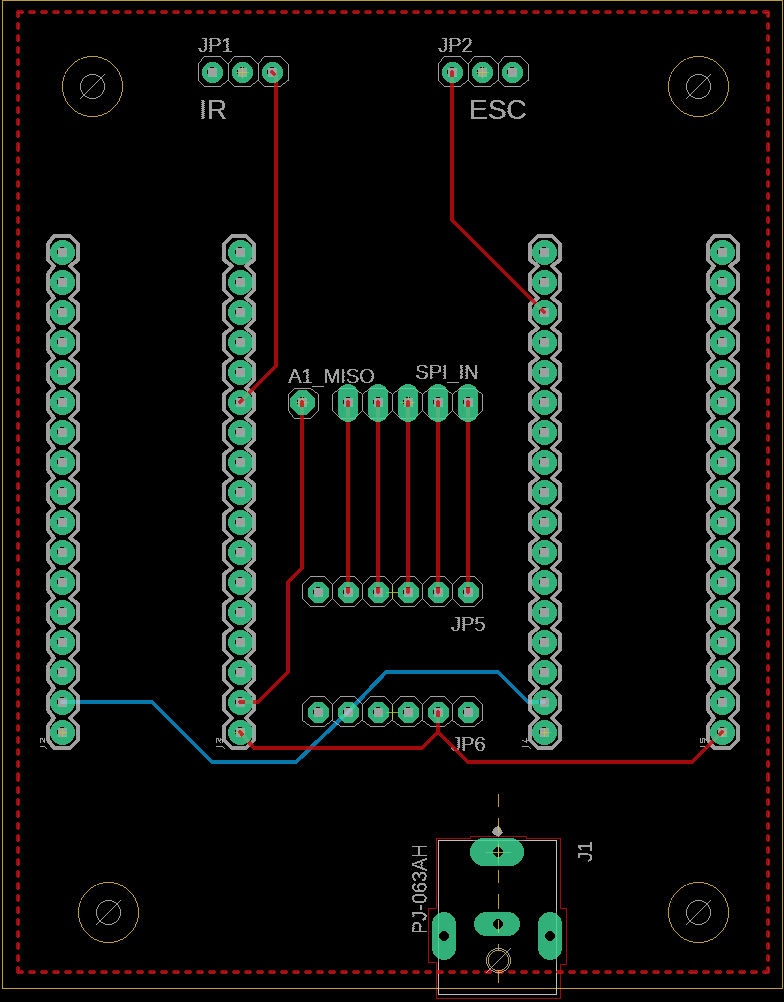
\includegraphics[width=0.3\textwidth]{borad_layout_ir_esc.png}
	\caption{Layout of the Board for speed sensor and ESC}
	\label{fig:board_layout_ir_esc}
\end{figure}

%-------------------------------------------------------------------------

\clearpage
\section{Implementation}

%-------------------------------------------------------------------------
\subsection{System overview}
maybe put communication diagram here

%-------------------------------------------------------------------------
\subsection{SDN network Implementation}

At the beginning of the project was floodlight that SDN controller framework we decided to work with. Under the project way was a lot of problem coming up to integrate floodlight on raspberry pi due to some java packages used in Floodlight was not supported, and it had difficulties to communicate with the SDN switches. This resulted in that another SDN framework was selected, and it was a framework called Ryu. Ryu was selected because it was well documented with some example code to start with, and it was developed in python, so it should be no problem with integrating it on a raspberry pi. 

The code for the Ryu controller is based on the example simple-monitor.py there the scripts requests information from the switches about how many ports that are used and the amount received and send traffic. The modification don to it is to save the received information so it can be presented in on a webpage.

To monitor the traffic load on the network was a webpage made to present the user with data. The webpage is developt from the provided network webpage included in Ryu. On the webpage, as shown in figure \ref{fig:webpage_sdn} is a table what presented the data that has been transmitted and received on each port, and the number of packages has been dropped. The web pages are designed to update itself every 10s to be updated with the latest information.  This has to do with the controller request new information from the switches every 10s.  In the bottom of the webpage is a picture of how the network is configured. 

\begin{figure}
	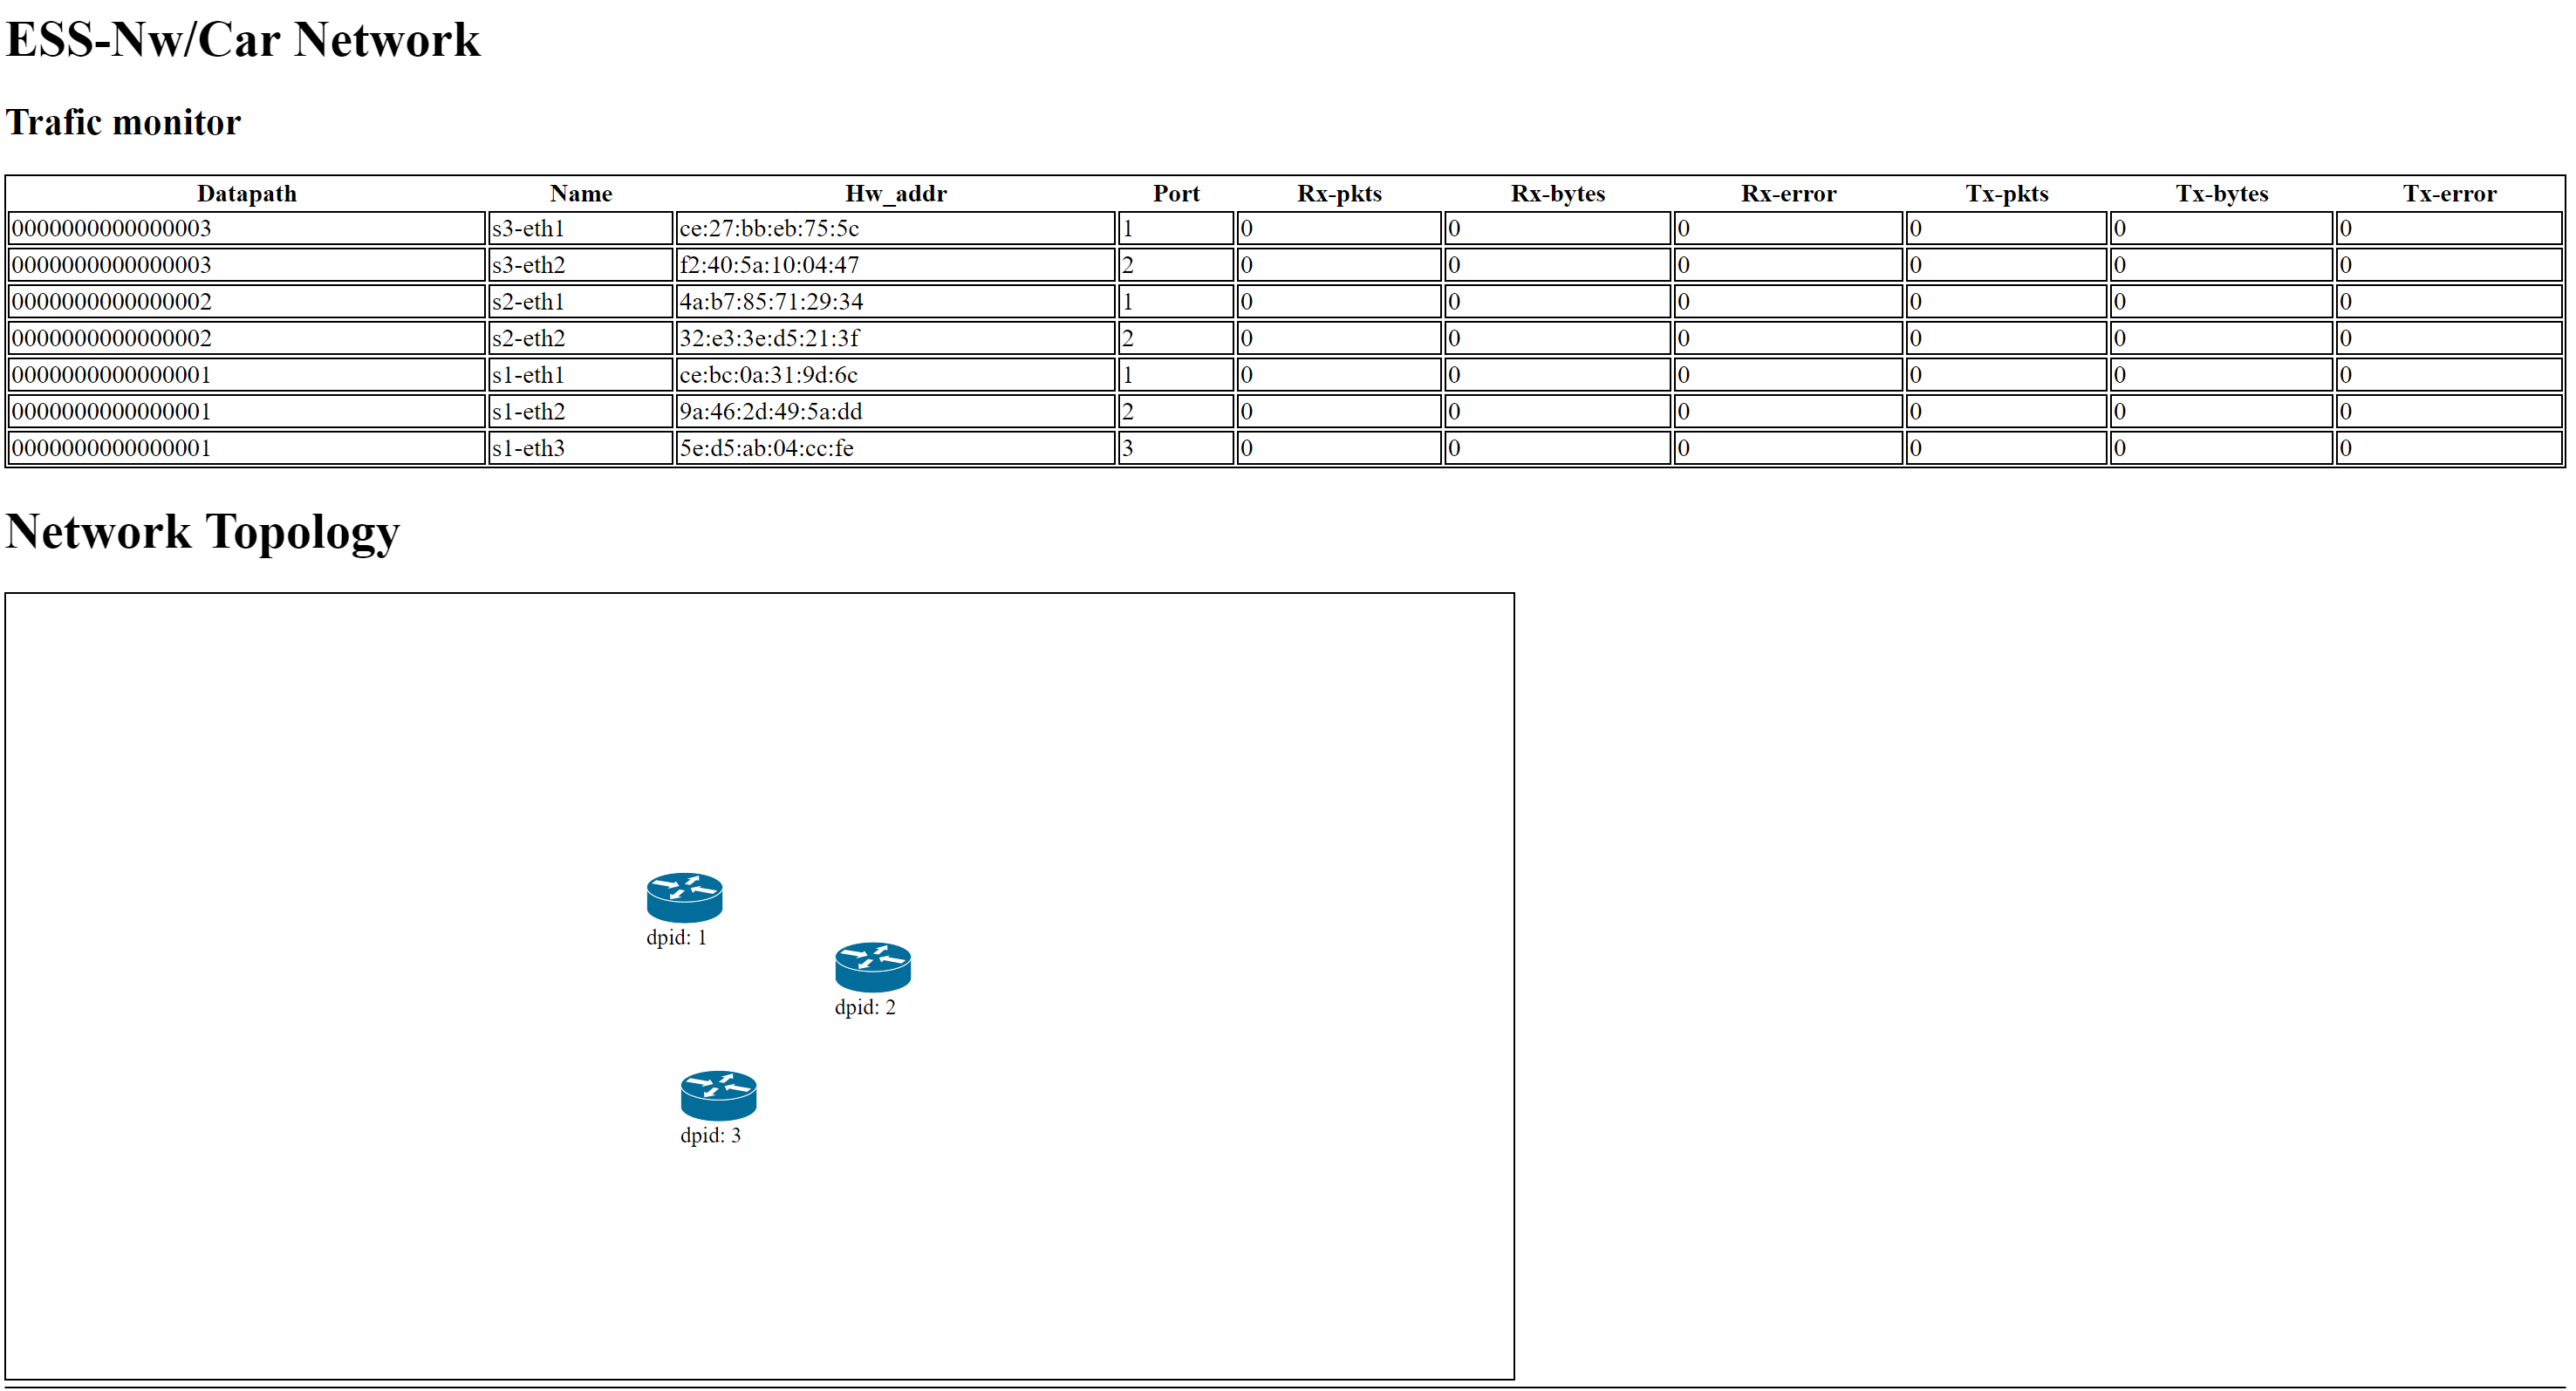
\includegraphics[width=0.3\textwidth]{webpage.PNG}
	\label{fig:webpage_sdn}
	\caption{Webpage to monitor the SDN network}
\end{figure}


%-------------------------------------------------------------------------
\subsection{Interprocess communication}
To increase coherency and decrease coupling in the software architecture we chose to have several running processes on all of the beaglebones. Each process is focused on doing a fewer amount of tasks which makes development easier. An example of this is the BeagleBone connected to the speedometer and the motor controller. It is running one process whose task is to talk to two Arduinos over SPI, where it sends information to the motor Arduino and gathers information from the speedometer Arduino. The other process on the BeagleBone is running the VsomeIP application. It is clear that these processes need to communicate with one another as the first process needs to access the ethernet.

The interprocess communication is implemented using shared memory. This is a POSIX concept which is implemented in Linux where more than one process can load in the same physical memory blocks into their own private virtual memory space. This is done using a few system functions and the operating system will make sure to take care of all the complex implementations.

Using shared memory is not enough, the communication also needs to be defined such that all processes using the shared memory knows how it should be used. For the cars specific need a circular buffer is implemented on the shared memory. This is to have a type of flow control where the values in the buffer are always relatively fresh. If a FIFO buffer was used instead and it is not being read as often as it is written to  the buffer might overflow, whereas now the oldest values in the buffer is just overwritten. When values are read from a FIFO the oldest value is always read first. There is no guarantee of how old this data is and might not be usefull to read any longer. With a circular buffer it is possible to adjust the size such that the oldest value is always relatively fresh.


\subsection{Communication between Beaglebone and Arduino ?}
%%%%%%%%%%%%%%%%%%%%%%%%%%%%%%%%%%%%%%
% SPI introduction in literature review, pros over UART
%TODO reference to the simple gpio library (github page)
% NOT SURE: PUT simple gpio lib to management chapter
%%%%%%%%%%%%%%%%%%%%%%%%%%%%%%%%%%%%%
As the Beaglebone only supports to be the master in a SPI connection, so we have two beaglebones with SPI configurations and each of them has two Arduino slaves. One Beaglebone has two spi devices: SPIDEV0 and SPIDEV1, and the SPIDEV1 device is disabled initially but is used for HDMI interface. 

In order to have one SPI device on Beaglebone connecting to multiple Arduino slaves, we use a third party C++ library called SimpleGPIO which enables us to use other general purpose pins as slave select of the SPI connection. Before we start communication with a specific Arduino slave, the corresponding slave select will be set to low, then we get access to that Arduino slave.

In the Arduino side, the communication request from the Beaglebone is treated as an interrupt. Then the Arduino writes/reads to/from the Serial Peripheral Data Register (SPDR). 
\subsection{Sensors}
Three categories of sensors are implemented in the prototype vehicle to monitor its surrounding environments. Data from distance sensors and speed sensor will be sent to an Arduino initially, then sent to corresponding Beaglebone. Data from Pi Camera will be sent to the Raspberry Pi which is directly connected to the main network.
%-------------------------------------------------------------------------
\subsubsection{Ultrasonic sensor}
%%%%%%%%%%%%%%%%%%%%%%%%%%%%%%%%%%%%%%%%%%%%%%%%%%%%%%%%%%%%%%
% put why we choose HC-SR04 in other chapter, e.g. methdology
%%%%%%%%%%%%%%%%%%%%%%%%%%%%%%%%%%%%%%%%%%%%%%%%%%%%%%%%%%%%%%
To get data from HC-SR04, a short 10\textmu s pulse should be supplied to the trig pin of ultrasonic sensor, then the sensor will send out an 8 cycle burst of ultrasound at 40 kHz and raise echo. The echo signal we get is a distance object which is pulse width and the range of the signal is in proportion. 

An Arduino Micro handles both the generating the trig pulse and interpreting the echo signal. The Arduino will set the output pin to low, wait for 5ms, set the pin to high, wait for 10ms, set the pin back to low. This is the process of generating the trig pulse. After the Arduino sends out the trig pulse, it waits for 2 ms, then reads the value from the pin connected to sensor's echo pin. The last step is convert the received value to distance in unit of centimeter.

%TODO distance sensor working process figure

\subsubsection{Reflective object sensor}
A reflective object sensor consists of an IR-diode and an IR-receiver encapsulated in a houseing and detects reflective material (such as white paper) placed perpendicular in front of its front. The sensor chosen was the OPB715Z from TT electronics and is characterised to detect white paper up to a distance of 12.7mm.

The relfective object sensor was used to implement the cars speedometer. It works as a type of RPM meter which measures the rotation of an object over a time period. It is then possible to extract the speed of the rotation given the amount of rotation and the time period. To gather the amount of rotation the sensor is mounted on the axis of the wheel aimed towards the inside of the wheels rim. A number of strips of reflective aluminum tape have been mounted on the inside of the rim, with equal distance between them, to trigger reliable readings from the sensor. The physical setup is depicted in figure \ref{fig:speedometer}.

The sensor is connected to an Arduino using a Vcc, a ground and a data cable. The data cable continously transmitis digital information by either being logical zero equalling ground when no reflective obejct is detected and a logic one equalling Vcc (5V) when a reflective object is detected. It is therefor needed that the sensor is connected to an arduino that processes this data further. The arduino is triggered by an interrupt when the sensor detects a reflective strip attached to the wheel. The arduino then fetches the amount of time since the last interrupt and calculates the current velocity.

One limitation with this approach is that the speedometer becomes less acurate the slower the car is going. An analysis of the case of standing still shows that a relfective strip inside the tire will never pass the sensor. This could be solved by allowing some amount of time to pass without detecting a strip before assuming that the acutal speed is zero. It is however impossible beneath some speed to distinguish if the car is traveling very slowly or if it is standing still. To tackle this problem a total of ten strips were added to the inside of the rim such that strips will be detected more often thus increasing the accuracy of the speedometer at slow speeds. A new speed is also calculated each time a strip is detected which is something that has its trade-offs. It may result in more noise when travelling at higher speeds, but by instead waiting for more than one strip to be detected it becomes type of running-average filter which helps to reduce noise that may be induced by uneven spacing of the reflective strips.

    Using the timing data and the physical propertis of the wheel the velocity is calculated according to equation (\ref{eq:velocity}) where steps is the amount of reflective strips detected since the last calculation and the stepdistance is the physical distance traveled between two strips. The result can then also be manipulated to get the desired unit, which in this case was centimeters per second. The calculation is done on the Arduino before transmitted to a BeagleBone via an SPI interface. Since SPI transmits one byte of information at a time, and this specific implementation is limited to transfer no more, the maximum speed that can be measured is 255cm/s before the value wraps around.

\begin{figure}[]
	\centering
   	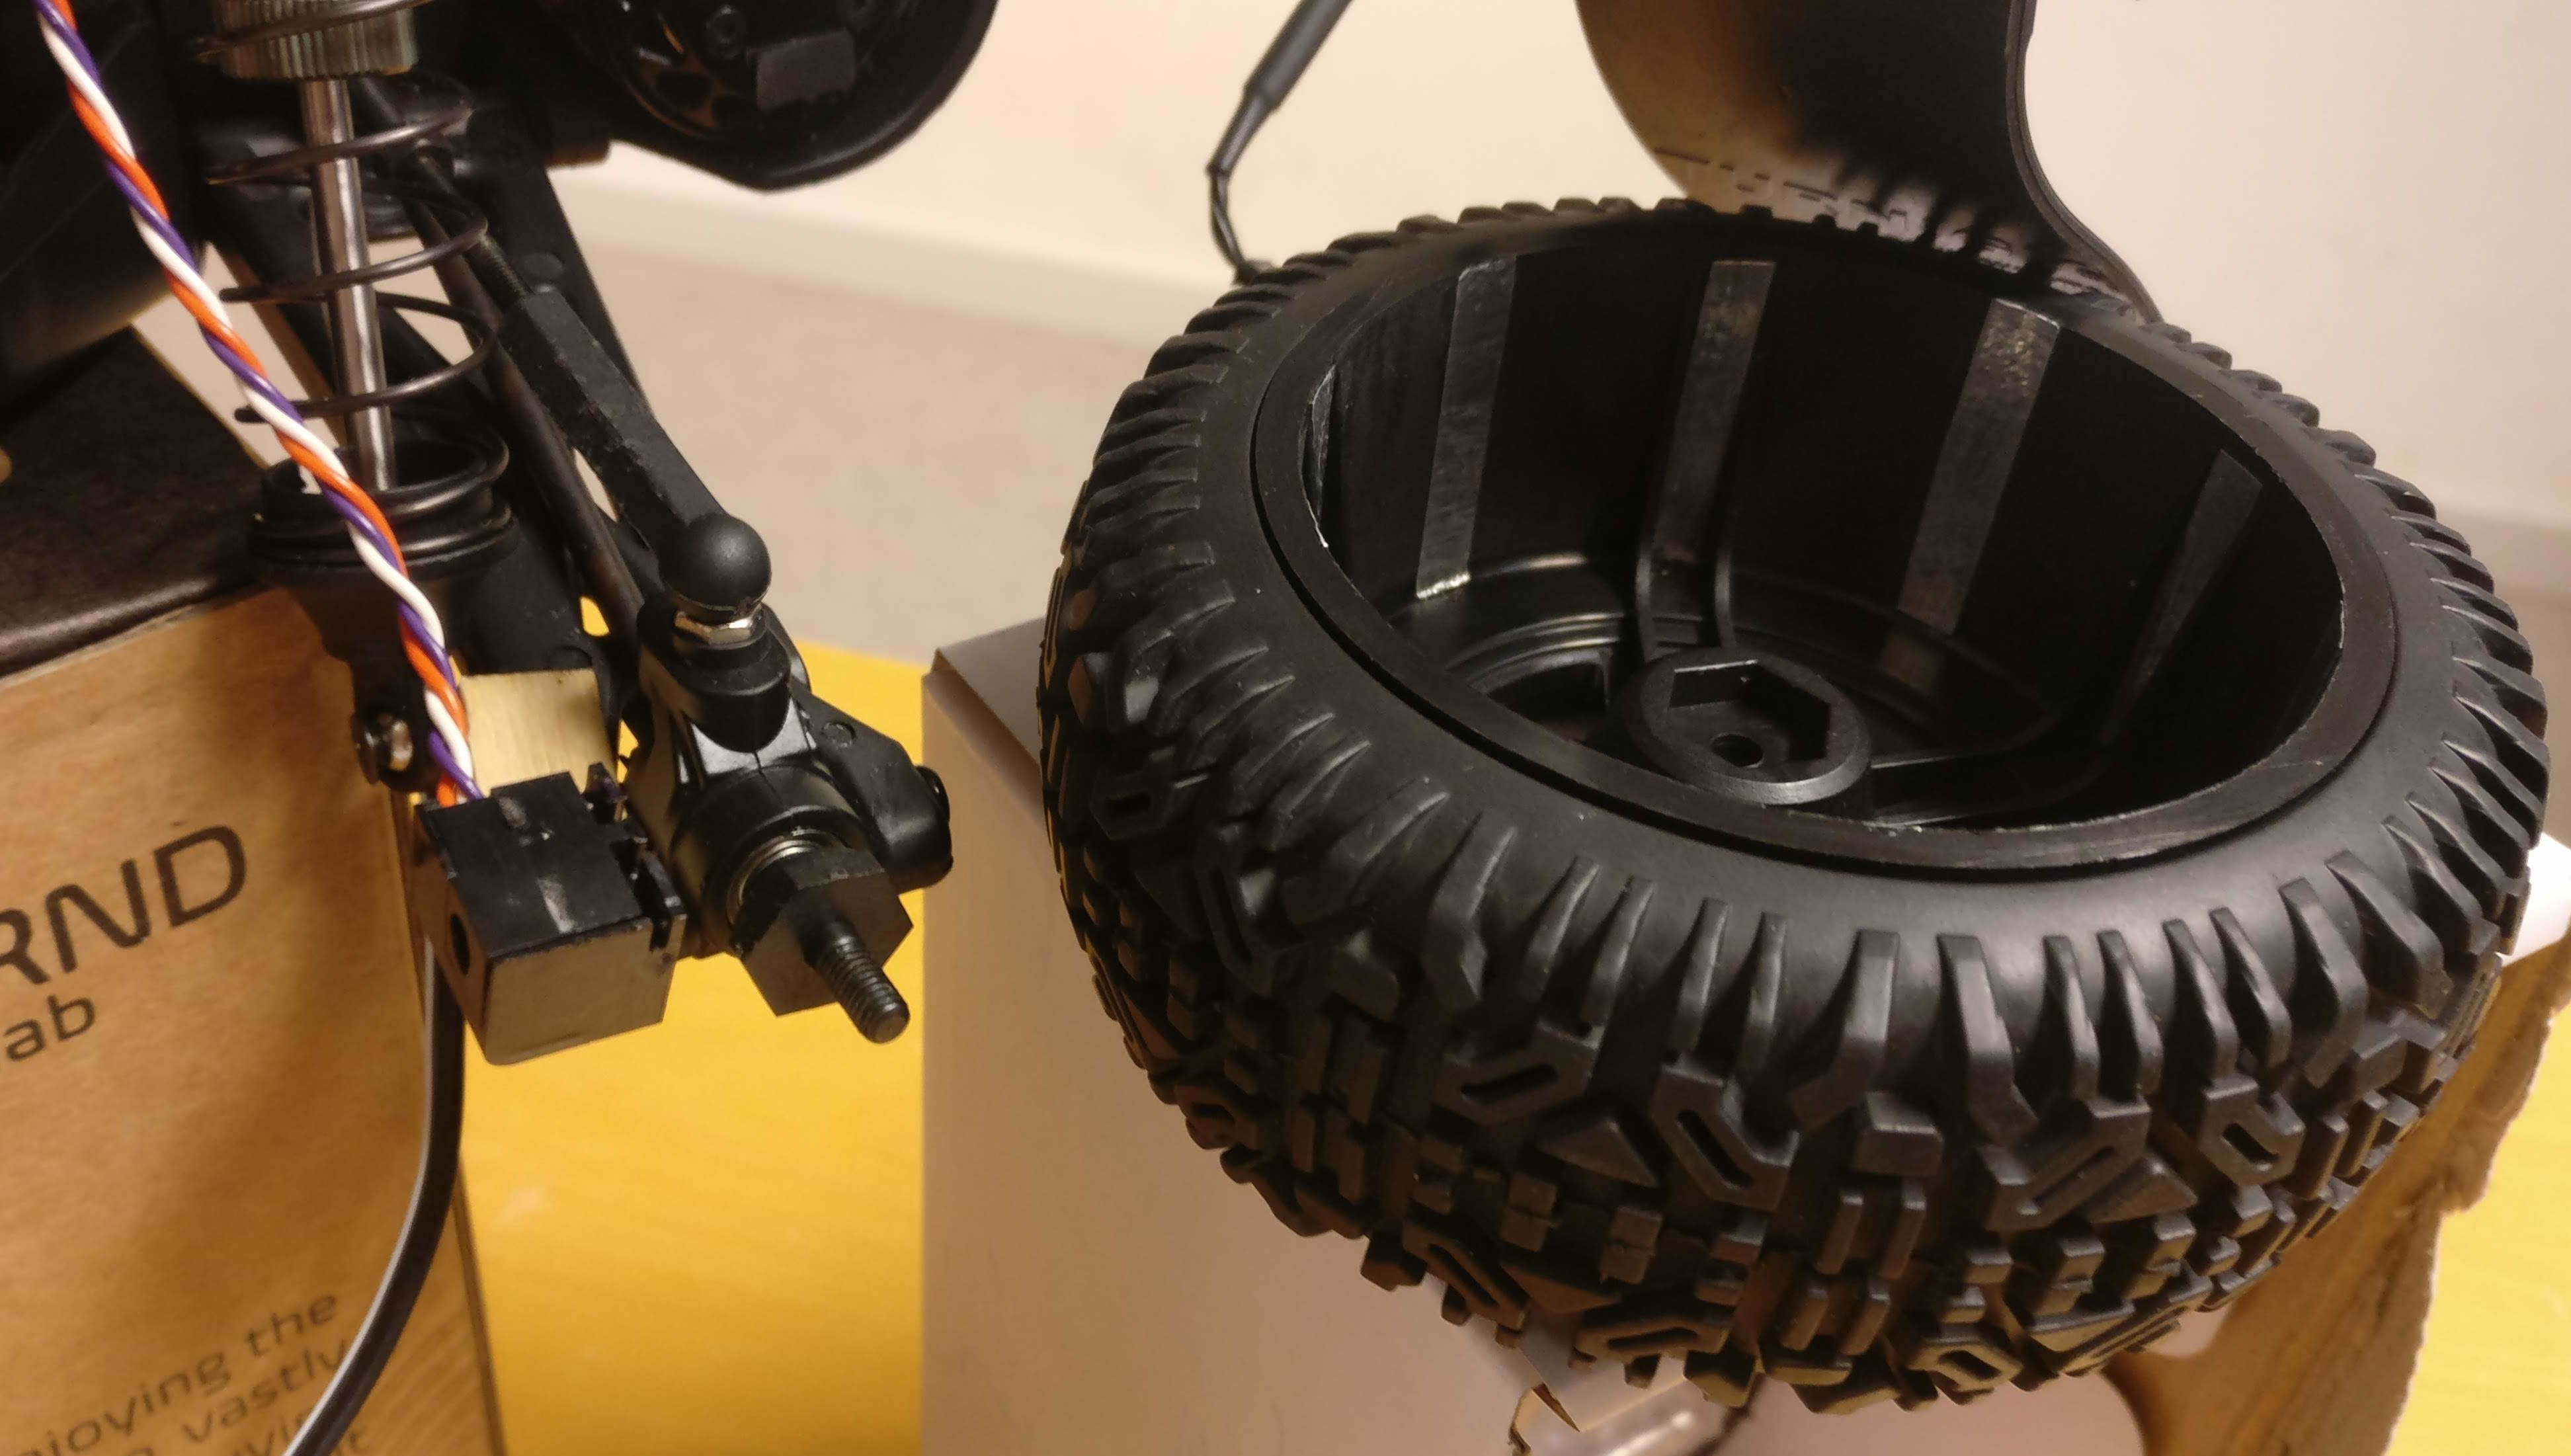
\includegraphics[scale=0.5]{speedometer.jpg}
   	\caption{Sensor mounted to the wheel axis on the left and the reflective strips mounted inside the wheel on the right.}
    \label{fig:speedometer}
\end{figure}

\begin{equation}
    velocity = \frac{(steps*stepdistance)}{time}
    \label{eq:velocity}
\end{equation}

An idea for future implementation would be to dynamically adjust the amount of reflective strips that needs to be detected before calculating the speed depending on the current speed to both increase accuracy when going slow and fast. Future implementations couls also allow for more than just one byte of data to be transfered over the SPI, not limiting the max read speed without loosing accuracy.

\subsubsection{Pi Camera}
In Pi’s vision part, we tried to compare the performance of two different methods, which are object detection based on neural network and traditional computer vision technique using OpenCV.

To improve the accuracy of the deep learning part, we investigated if transfer learning techniques can be applied on the specific problem. On the other hand, to improve the real time performance, we think that model compression should be evaluated to fit the network into a smaller and faster net topology, without losing significant accuracy. 

We have chosen several different pre-trained network to meet our demands. Including “shape-detection” network and MobileNet. Shape detection network is a very simple and fast deep neural network which simply detect the shape of the object. But in the real test we found that this network is not robustness enough for our fast-moving scene since it frequently predict wrong results.

Apart from using pretrained neural network, we have also train a Convolutional Neural Network to do the classification using online open source labeled dataset. The German Traffic Sign Detection Benchmark (GTSDB) is a labeled dataset for AI researchers who work on computer vision-based driver assistance. It contains 900 images, which divided in 600 images for training and 300 images for testing process. figure \ref{fig:GTSDB1} and figure \ref{fig:GTSDB2} are example images in dataset.
\begin{figure}[]
	\centering
   	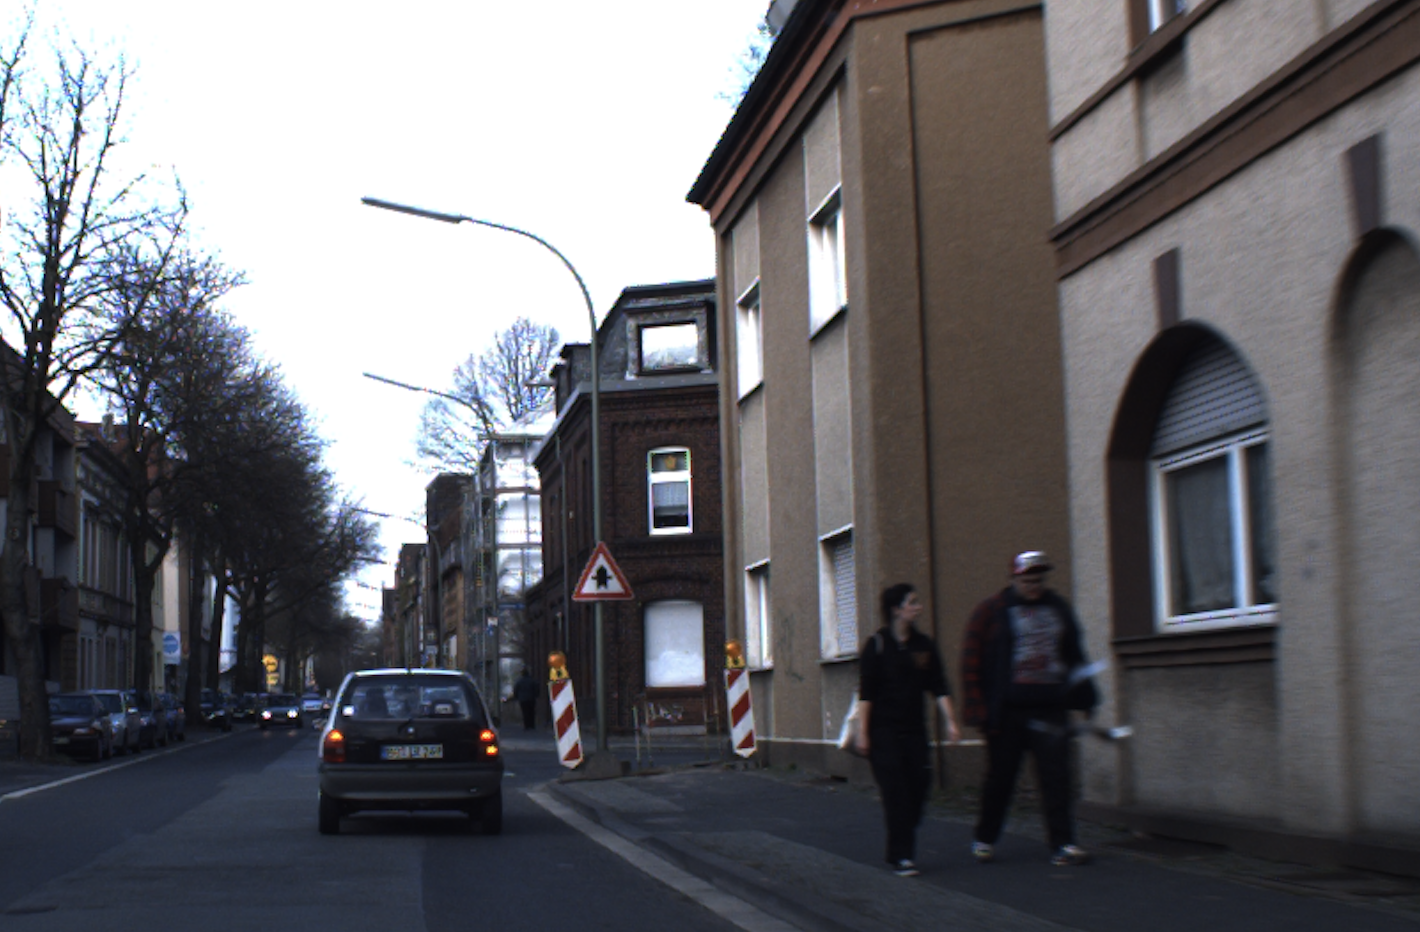
\includegraphics[scale=0.3]{GTSDB1.jpg}
   	\caption{Example image from dataset}
   	\label{fig:GTSDB1}
\end{figure}

\begin{figure}[]
	\centering
   	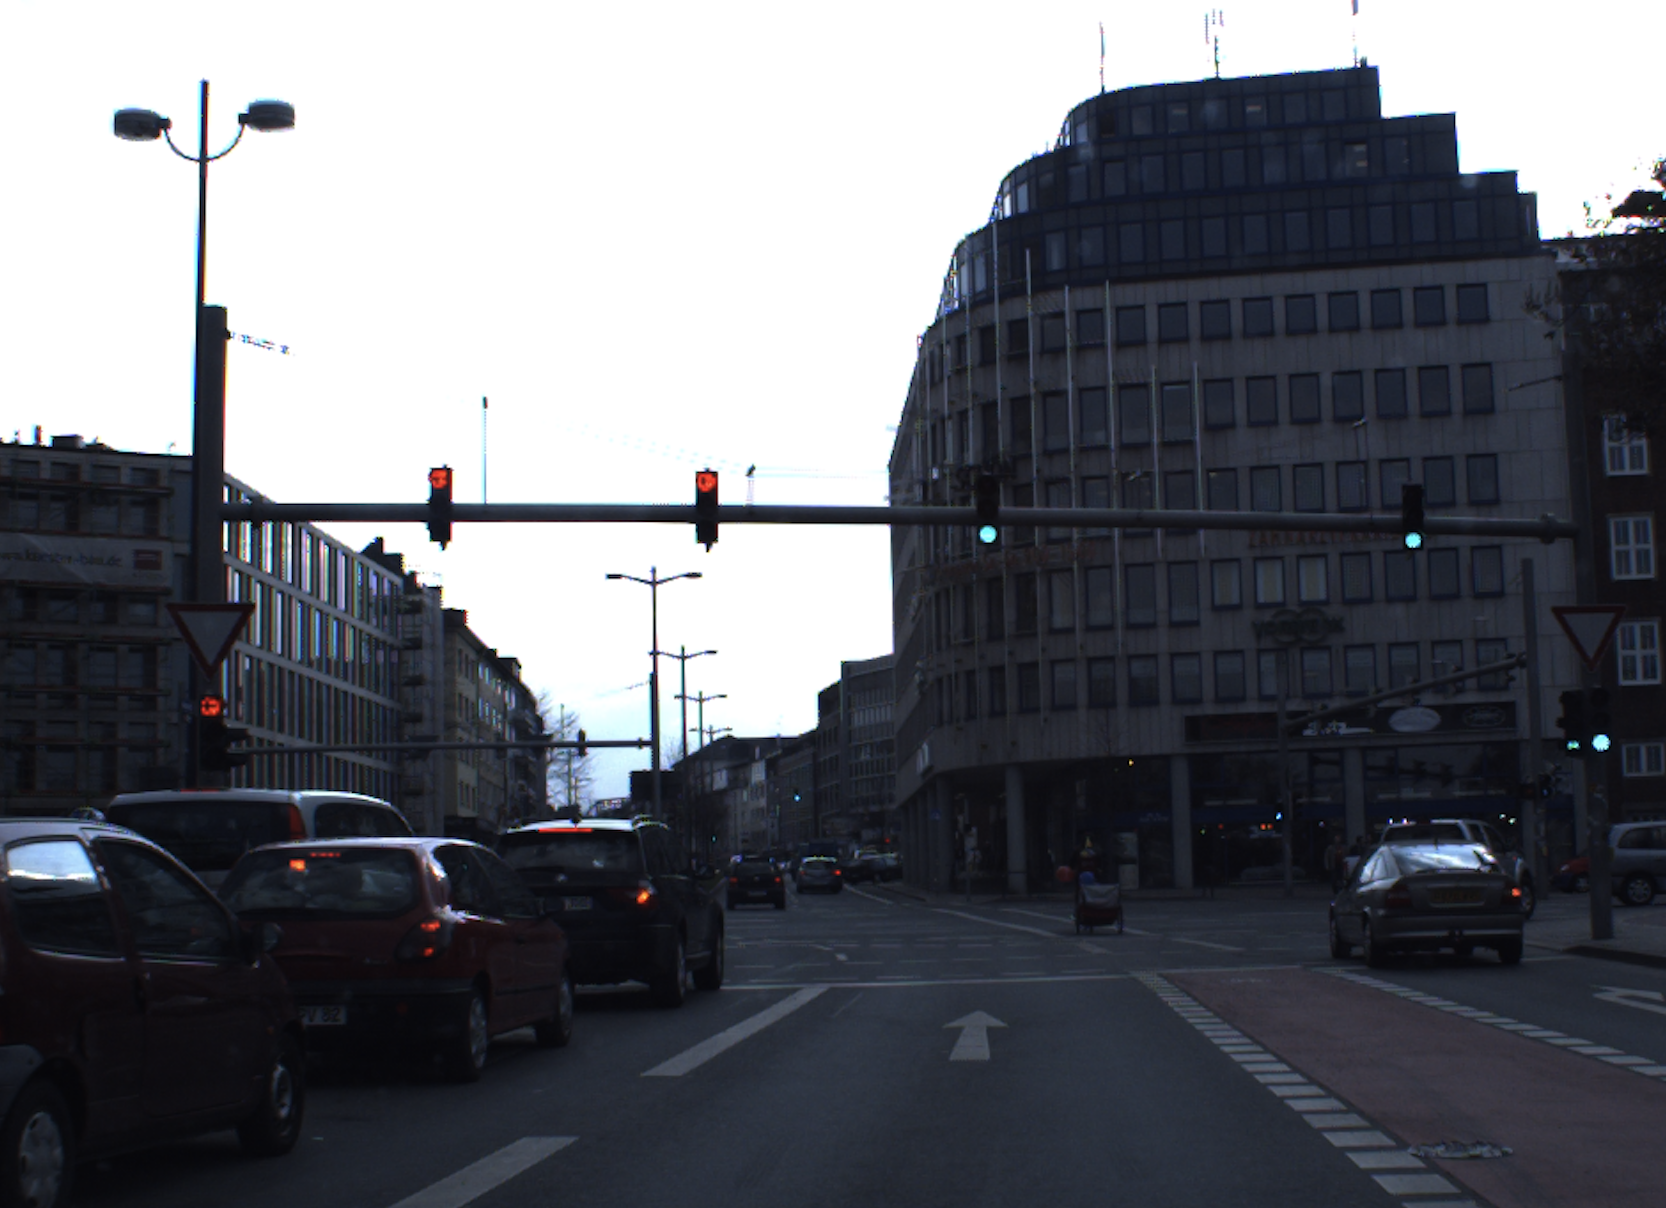
\includegraphics[scale=0.3]{GTSDB2.png}
   	\caption{Example image from dataset}
   	\label{fig:GTSDB2}
\end{figure}
In the neural network that we trained ourselves, we first down-sampling the images to 32*32 as input, then use 4 convolutional layers to extract the image features and use additional residual stack and dense layer to do the classification. The structure of neural network is shown in figure \ref{fig:network}. The overall accuracy is good using these network because of the powerful prediction ability of DNN. However, the model is not that fast to deal with our car and it takes a lot of time for this network to process one video frame and produce output. 

\begin{figure}[]
	\centering
   	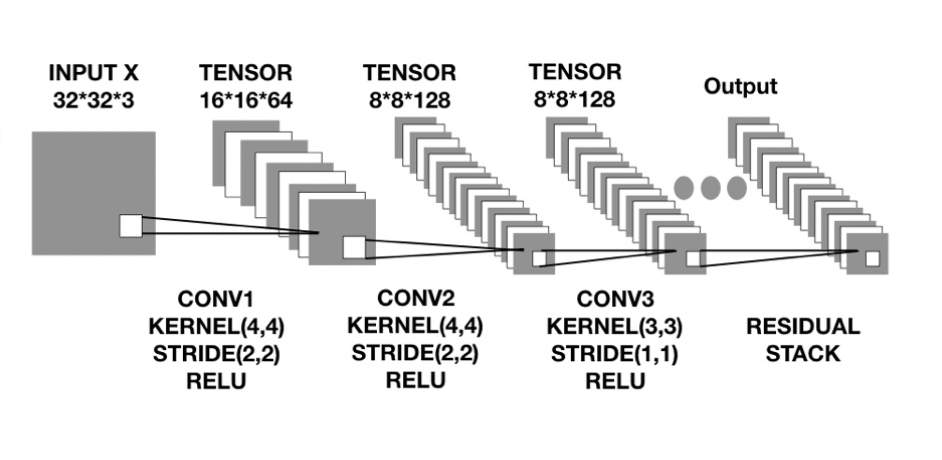
\includegraphics[scale=0.6]{network.png}
   	\caption{Structure of network}
   	\label{fig:network}
\end{figure}

Finally, we decided to use the technique of transfer learning to apply MobileNet on RPI, which is an efficient model for mobile and embedded vision applications. The speed remains slow although multiprocessing and hardware acceleration have been carried out to improve.

By using OpenCV’s DNN module to apply a pretrained object detection network. Then we are able to pass input images through the deep neural network and get a output image with bounding box of specific object and label.

The distinct feature of MobileNet is that the core layer of it is depthwise separable filters. Depthwise separable convolution have different structure from a standard convolution since the standard one put both filters and combines as inputs and get outputs in a single step, whereas depthwise separable one separate these two into two different layers, one of them as filter and the other one for combining. This specific structure can largely reduce the computation cost and model size. The structure of these two convolution filters are demonstrated in figure \ref{fig:convolution1} and figure \ref{fig:convolution2}.

\begin{figure}[]
	\centering
   	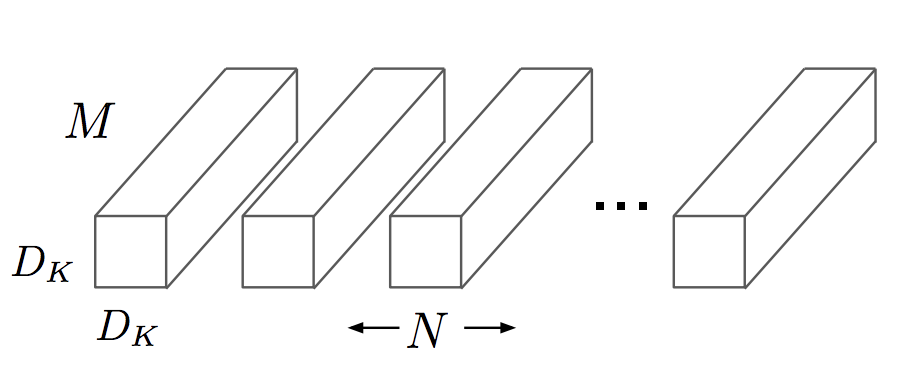
\includegraphics[scale=0.5]{convolution1.png}
   	\caption{Standard convolution}
   	\label{fig:convolution1}
\end{figure}

\begin{figure}[]
	\centering
   	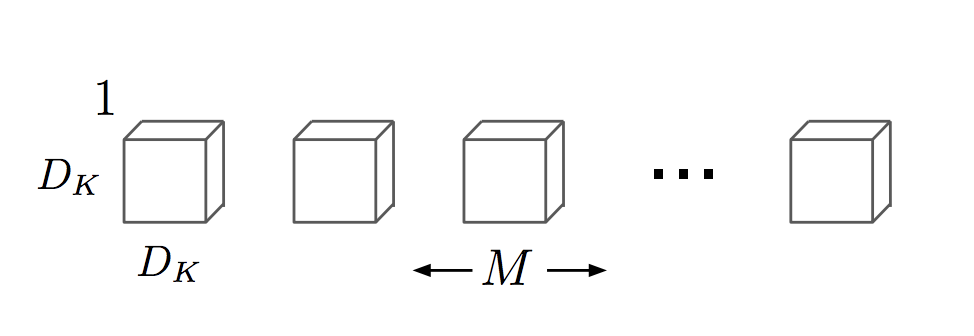
\includegraphics[scale=0.5]{convolution2.png}
   	\caption{Depthwise separable convolution}
   	\label{fig:convolution2}
\end{figure}
The layer of standard convolution and of depthwise separable convolution are shown in figure \ref{fig:convolution3} and figure \ref{fig:convolution4}. More details, figure \ref{fig:convolution3} shows a standard convolution layer, following by batch normalization and ReLU. Batch normalization makes the learning of layers in the network more independent of each other. It is a technique to address the problem that the distribution of each layer’s inputs changes during training, as the parameters of the previous layers change. The technique consists of adding an operation in the model just before the activation function of each layer. Then add a ReLU activation function, which is rectified linear unit to define the positive part of its argument and negative part of 0. Figure \ref{fig:convolution5}  shows the plot of ReLU.

\begin{figure}[]
	\centering
   	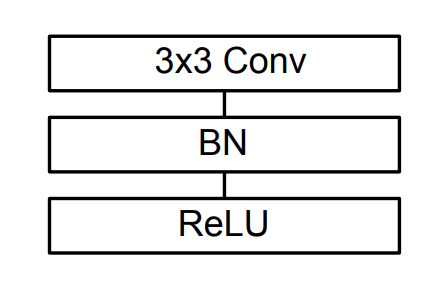
\includegraphics[scale=0.5]{convolution3.png}
   	\caption{Standard convolution layer}
   	\label{fig:convolution3}
\end{figure}

\begin{figure}[]
	\centering
   	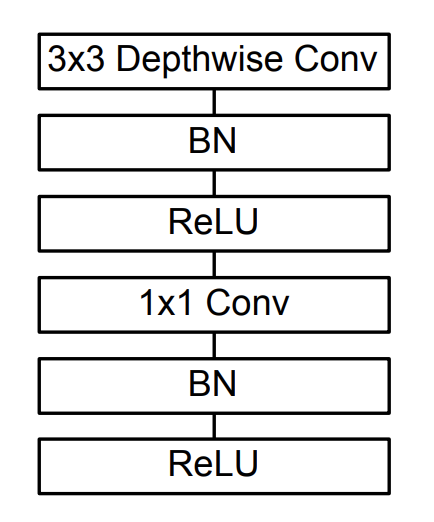
\includegraphics[scale=0.5]{convolution4.png}
   	\caption{Depthwise Separable convolution layers}
   	\label{fig:convolution4}
\end{figure}

\begin{figure}[]
	\centering
   	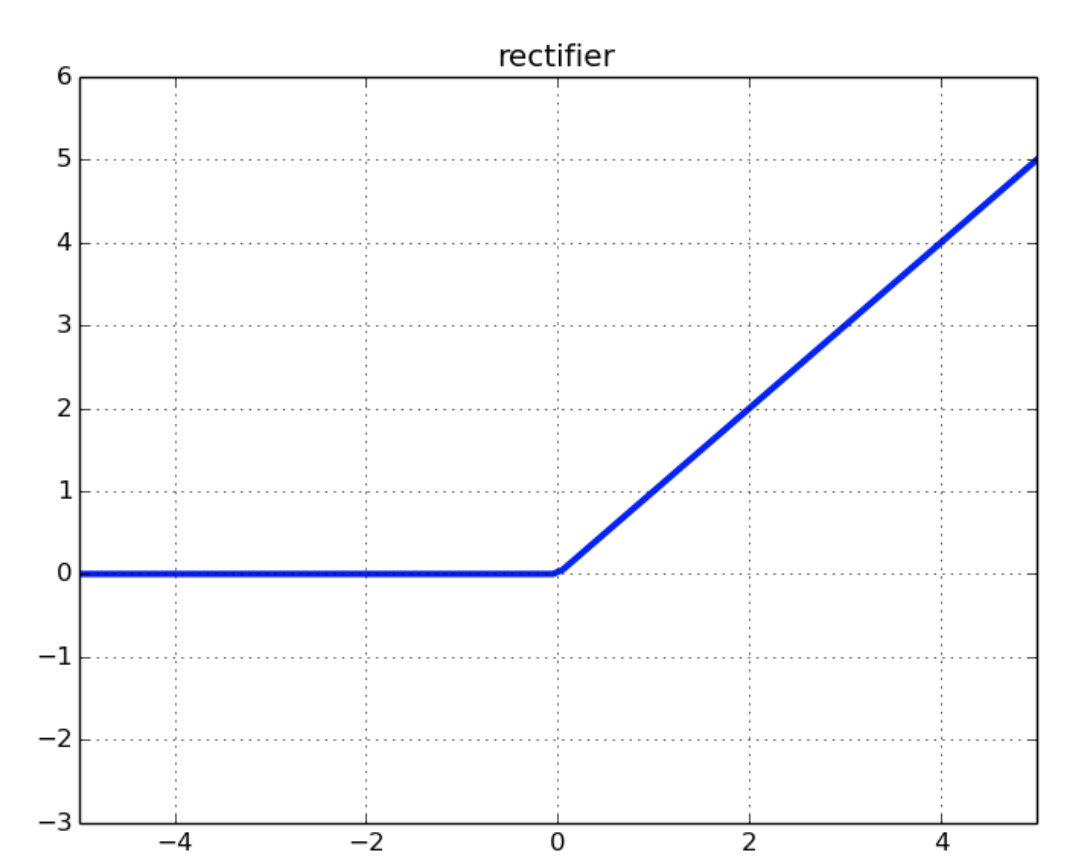
\includegraphics[scale=0.3]{convolution5.png}
   	\caption{plot of ReLU activation function}
   	\label{fig:convolution5}
\end{figure}

Figure\ref{fig:convolution4} describes depthwise separable convolution layers with 3 x 3 depthwise convolution and 1 × 1 pointwise convolution following by batch normalization and ReLU activation function after each of the convolutional layer.

Since we are working on source constrained device Raspberry Pi, we need to make the network simple and decrease computational cost, so we combined MobileNet with Single Shot Detector.

Additionally, in order to optimize the Raspberry efficiently and use sufficiently limited resource and memory on it when running neural network, we did some optimizations. We firstly applied hardware optimization which is to install optimized OpenCV complie. ARM NEON, as an optimization architecture extension for ARM processors is installed. It is used for faster video stream processing, image analysis and speech recognition that is exactly what we are look for in our application. This architecture can execute multiple processing in the pipeline by a single instruction. Besides, VFPV3 as a floating point optimization is also used. After the first stage improvement, we get a 30 percent speed increase since we have make full use of the 4× ARM Cortex-A53, 1.2GHz processor on Raspberry Pi, now the network is able to classify an object in 1.5 seconds. 

When it comes to second stage of optimization, multiprocessing is used to increase the speed of processing video stream. The I/O tasks, dislike CPU bound operations, always take lots of time and delay the process. So moving the reading of frames to a separate thread from processing the frame can obtain higher speed. Otherwise, every time I/O port access Pi camera, the main thread of script is blocked until the frame is captures and return to script. Multiprocessing can decrease the influence of I/O on CPU heavy application like video stream processing, especially in our real-time case. Now we can obtain a classification result in 1 second.

Moreover, there is a tradeoff between accuracy and output speed. In our application, we set a threshold for the output, in more details, only when the confidence score of detection result is high enough (above the specified threshold), the result can be output as a signal to steer the car. Otherwise, it will grab another frame and do the object detection for the other iteration. As a result, if the threshold confidence score of output increase, the output speed will decrease. 

After several tests, we found that it is not feasible to use DNN on the RPI because of the predicting speed, RPI has really limited computational capability and has no GPU that can be used to do the DNN-accelerate. After the mid-term, we decided to try another strategy which using the traditional computer vision technique offered by OpenCV.

Then we try to process video stream by using OpenCV. OpenCV has offered many traditional and start-of-art computer vision techniques which can be used . We tried several algorithms for the detection in our specific scenario, including SIFT/SURF keypoint detection, mog2 background subtraction, hough transform, and color detection using HSV space. Among these methods, we eventually chose color detection as our camera detection algorithm.

The color detection algorithm can be separated to different phases. First, we need to do the image pre-processing: we down sampling the images using different scaling factors since we want both processing speed and accuracy optimized. Then we transfer the RGB color space to the HSV color space to make the color easy to be identified. We define the upper and lower limits for pixel values to classify three colors. Then specify which pixels fall into specified upper and lower range by masking. Finally, we do the detection by comparing the HSV value of our processing frame and the pre-defined HSV color space value and output both the color and position information. The speed of color detection is fast and also accurate enough for real-time application.

To enable our model communicate with the VsomeIP perfectly and precisely. We tried several methods to connect Python program and C++ program, including using Google protocol buffers and RAM pipe transfer. We have to ensure that both of programs can communicate simultaneously without block. 

Apart from outputting the detection result and communicate with the SDN network, we have also tried to send the video stream through WIFI or Bluetooth to Android application so that we can know what the camera sees through smartphone. Although the real-time video stream can be sent to a web browser, the sending script cannot run when the detection script is running since they will block each other.


\subsection{Controlling actuators}
\subsubsection{Steering servo}
A servo motor was connected on the front axis of the car to enable steering. The servo is connected to an Arduino using a Vcc, a ground and a data cable. To control the servo motor, a pulse of varying length should be applied on the data cable. A Arduino library for servo controllers was used as it has definitions for these pulse lengths and was compatible with the servo motor used in the project.

One issue with the servo motor mount was that a direction change required the servo motor to turn a bit before it had any effect on the steering axis. This issue was fixed by changing the software implementation such that a direction change added or removed from the output pulse length.

\subsubsection{Motor ESC}
The motor mounted on the car is a \textit{TrackStar 17.5T "Outlaw" Sensored Brushless Motor V2} connected to a \textit{HobbyKing® ™ X-Car 45A Brushless Car ESC}. The ESC is connected to an Arduino using the RX signal and ground cable only.

There are a few steps needed to setup the ESC before it can be controlled by the Arduino. For the set up in this project, follow these steps:
\begin{itemize}
	\item Connect the RX signal and ground pin to the Arduino
	\item Load an Arduino program that allows you to manually send PWM signals on the signal pin. The program in mind uses the Arduino servo library function \textit{writeMicroseconds} and the PWM signal values will be defined according to the input values of that library function.
	\item Start the Arduino program but keep the ESC off
	\item Send a PWM signal of 2000
	\item Hold down "set" button on the ESC switch and switch it on while still holding down the button
	\item Wait for a solid orange light
	\item Release the "set" button on the switch and wait for a solid red light
	\item Send a PWM signal of 700
	\item Wait for a solid orange light
	\item Send a PWM signal of 1000
	\item Wait for a beep and for the lights to turn off
	\item Switch off the ESC
	\item The set up is complete. When switching on the properly set up ESC, make sure that there are no PWM signals higher than 1000 sent on the data pin.
\end{itemize}

The ESC has a safety measure for when the motor PWM is set to anything higher than \textit{neutral} (a pulse width of around 1000 microseconds), and the motor is too weak to carry the load and thus will not spin. In this case, the ESC will not listen for any other PWM signal other than \textit{neutral}. Once a \textit{neutral} PWM signal is sent for a couple of milliseconds, the ESC will start handling higher PWM signals again. The Arduino program running the motor has means of dealing with this case.

The Arduino program reads data for target speed and current speed through an SPI interface. This interface sends one byte at a time, where the most significant bit defines if the data is for target speed or current speed. This datastructure puts a limit on the values as there are only 7 bits left for data. The data is defined as 2 centimeter per second to increase resolution; sending a 10 would mean a speed of 20 centimeters per second. This allows the controller to read and maintain speeds of at most 255 centimeters per second with the only limit being the frequency of the speed sensor. 

The Arduino prgram has two possible implementation of speed keeping. To switch between these, one has to change a line in the source code. One implementation is a direct translation from target speed to motor pwm. If the pwm requirments for reaching a speed would change, this translation would not longer be valid. Driving on a flat surface would still be fine. The other implementation uses a PID controller which reads the current speed from the SPI. As the closed loop with data through SPI over two nodes, the data will be delayed by a couple of milliseconds, but tuning the PID parameters can result in a good PID controller.

A future implementation could focus on lowering the delay over SPI and tune the PID parameters properly. Sending multiple bytes over SPI at once would also remove the need of scaling the data before sending, and increase the resolution by at least one bit.

\subsection{Assembly of the car}


The platform pieces are achyle plastic and were cut via a laser cutter, the schematic for the pieces was exported from the 3D model to Illustrator to be sent to the laser cutter. The result of it is shown in figure \ref{fig:3d_platform}. The platform was mounted via board spacer of different sizes to mount the levels together. All the devices on were mounted via screws and nuts to keep them in place. 


\begin{figure}
	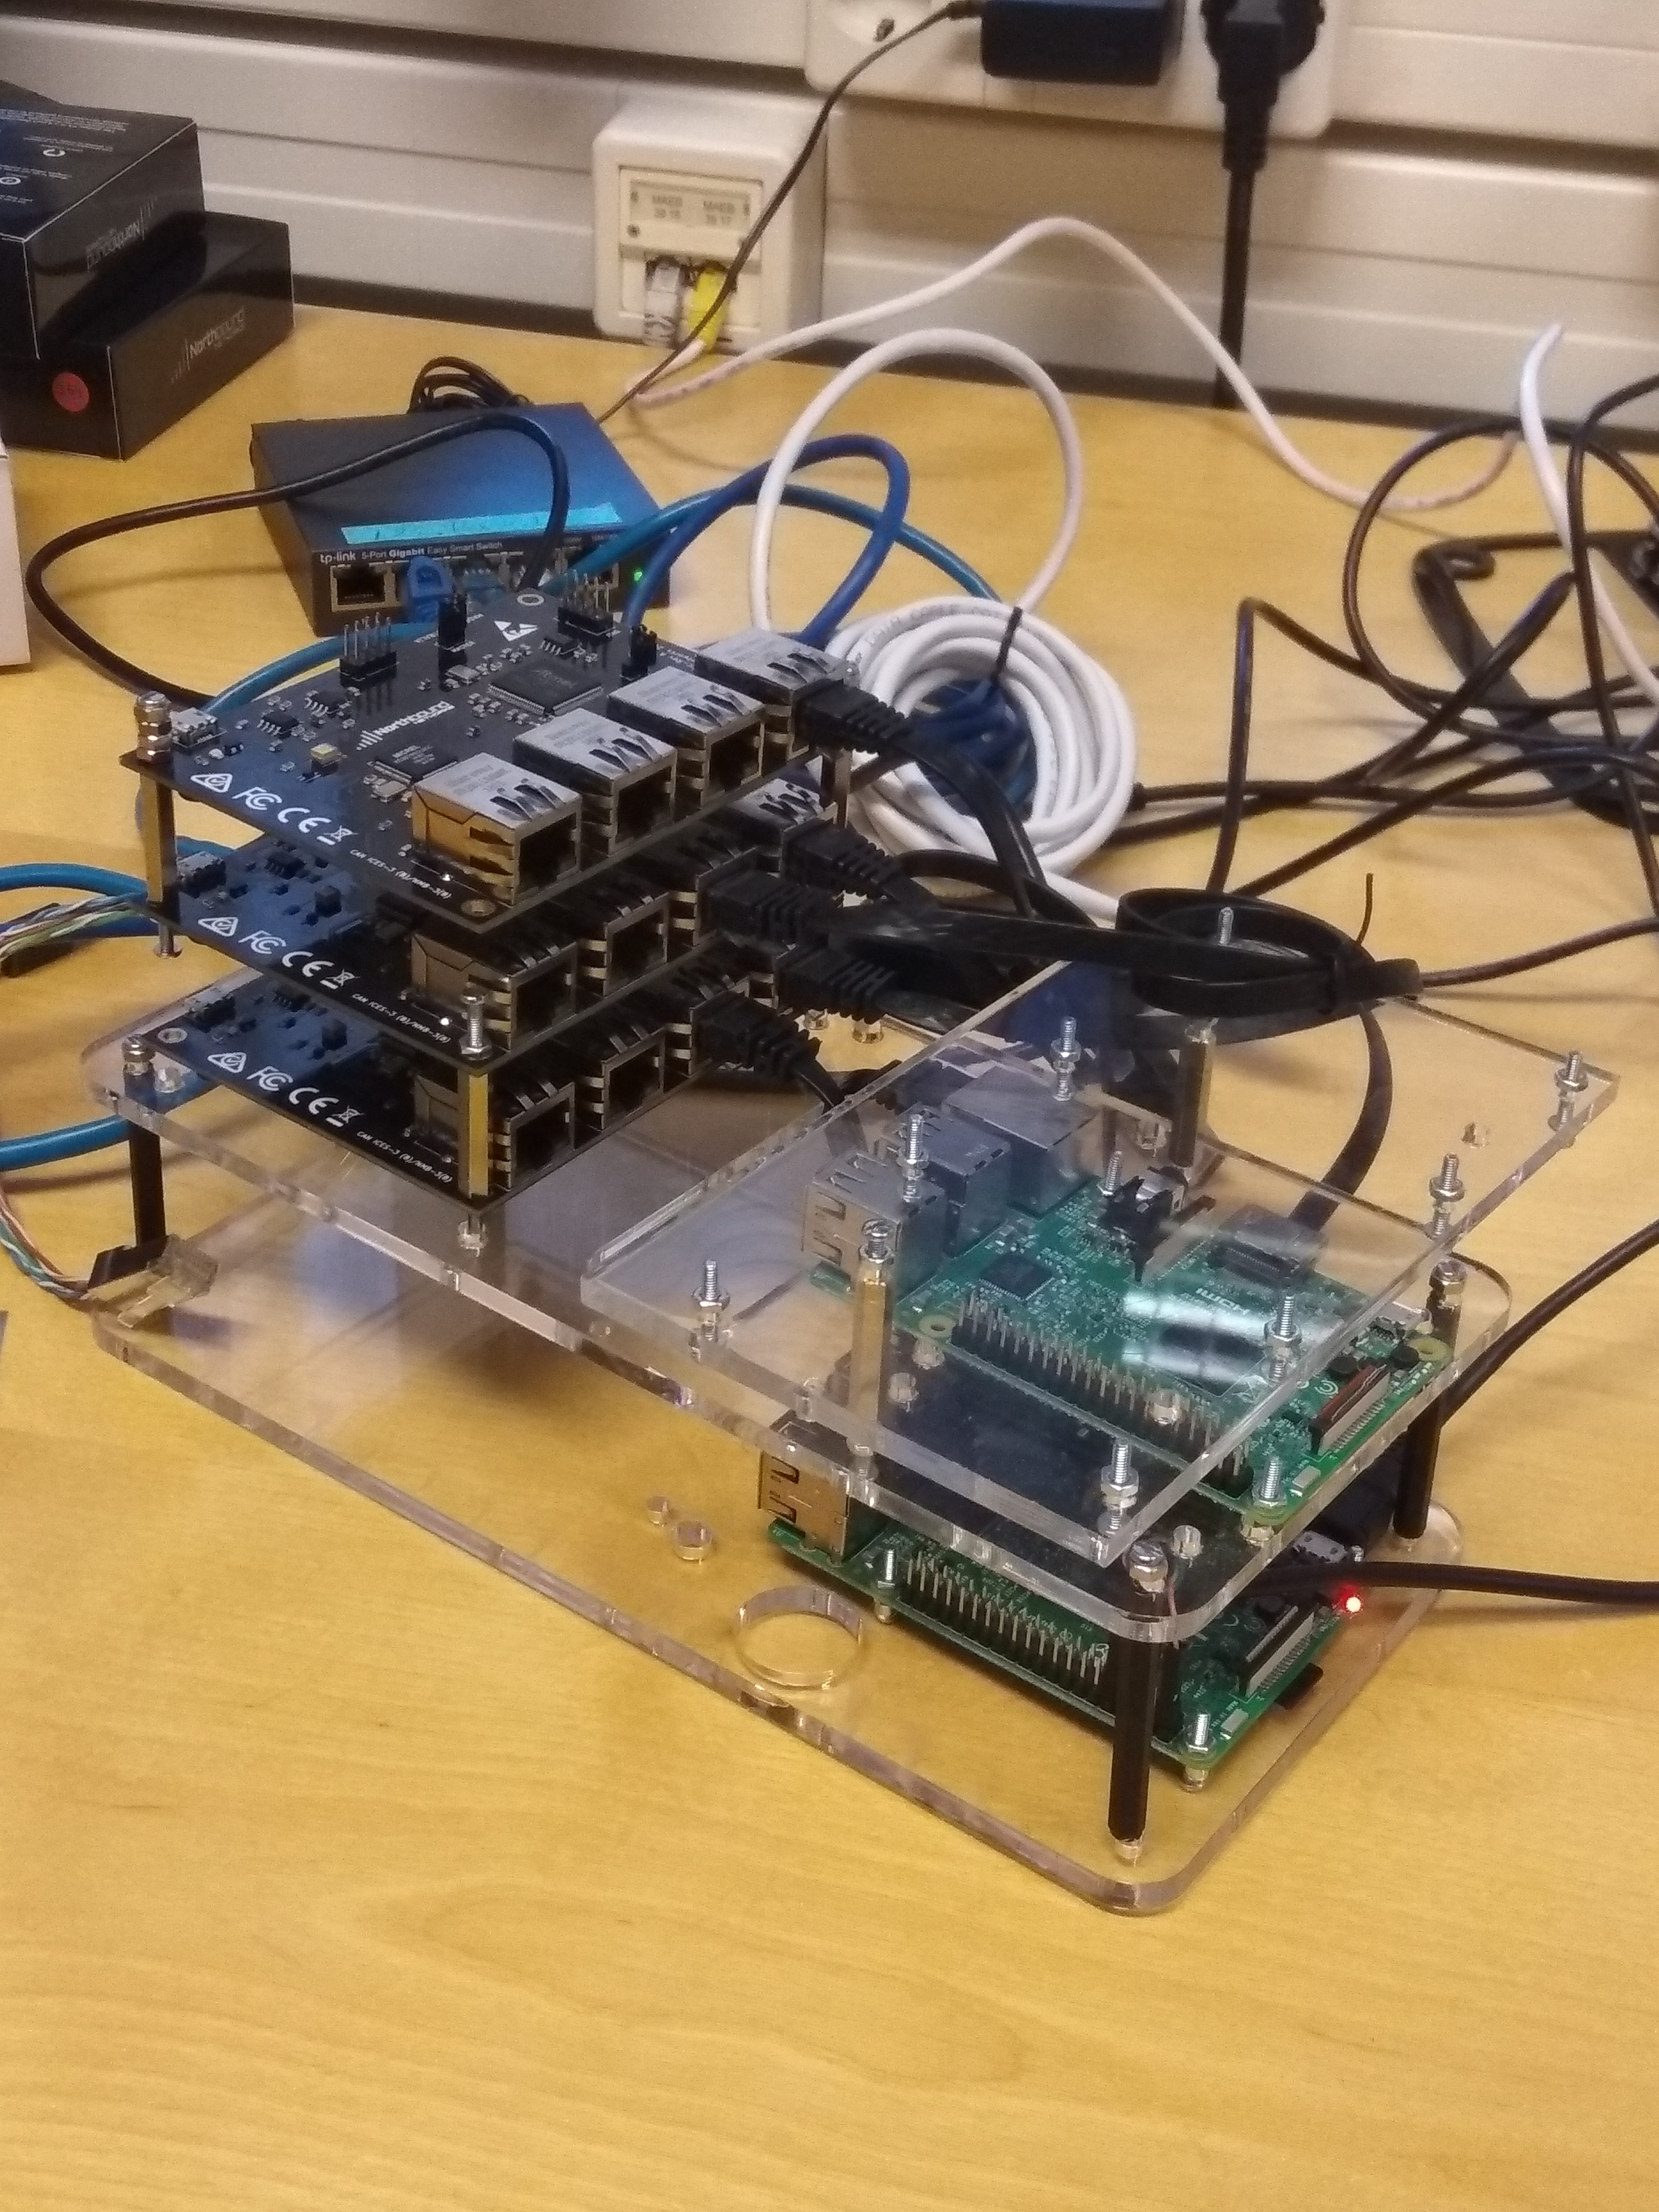
\includegraphics[width=0.3\textwidth]{platform_assembely.jpg}
	\caption{Platform}
	\label{fig:platform_ass}
\end{figure}

The design of the platform was done to use PCB bards and not prototyping bards, this made the assembly of the car not to be as the idea was. This is because it was difficult to make the prototyping bards small and compact as you can do with PCB.  Two of the boards The power board and one of the Arduino boards were able to place in the targeted position but could not be mounted to the platform with screws but with cable ties. The other board had to be placed in front of the car due to it could not be fit at its target place because the power board and the Arduino board was too thick of the wiring on the boards. 
 

%-------------------------------------------------------------------------
\subsection{Power Supply and PCB}

The idea of was to order the PCBs from a company, but due to course regulation ware we not allowed to order PCBs from China, and companies in Europe were too expensive to order from. This resulted in what we could not implement the boost converter we hade design due to the milling machine in both prototype centre and in Mentorspace was broken and they could not mill the layout for the boost converter. Because the milling machines were broken could the PCB for the Arduinos also not be made. The only way we could continue with was to make the design on a prototyping board. 

The implementation on the prototype board was built from the same concept the PCB should have had, with USB-A ports cables to power the Arduino boards and external switch. The bard connects via a cable from the battery to a fuse, this fuse is implemented to protect the system if a short circuit happens. To solve the boost converter circuit did we buy a boost converter module MT3608 to receive a 9V. This module is not connected to the 5V level but instead to the to the 7.2V from the battery, to receive a current higher than 0.6A. To prevent previous years failure then they used the module, did we add the same solution to add an led with a resistor in series and $ 6.8\mu F$ in parallel to the output pins on the boost converter.

The Arduino boards hade also be made at prototyping board. They received the same functionality as the PCB version should have, but it takes larger space due to the cable wiring. This lead to one of the board could not be placed at its position on the platform. 

The result of the prototyping is shown in figure \ref{fig:board_ultra_steering}, \ref{fig:board_speed_engine} and \ref{fig:Power_board}. All of them has the functionality has the same PCBs should have had. 


\begin{figure}
	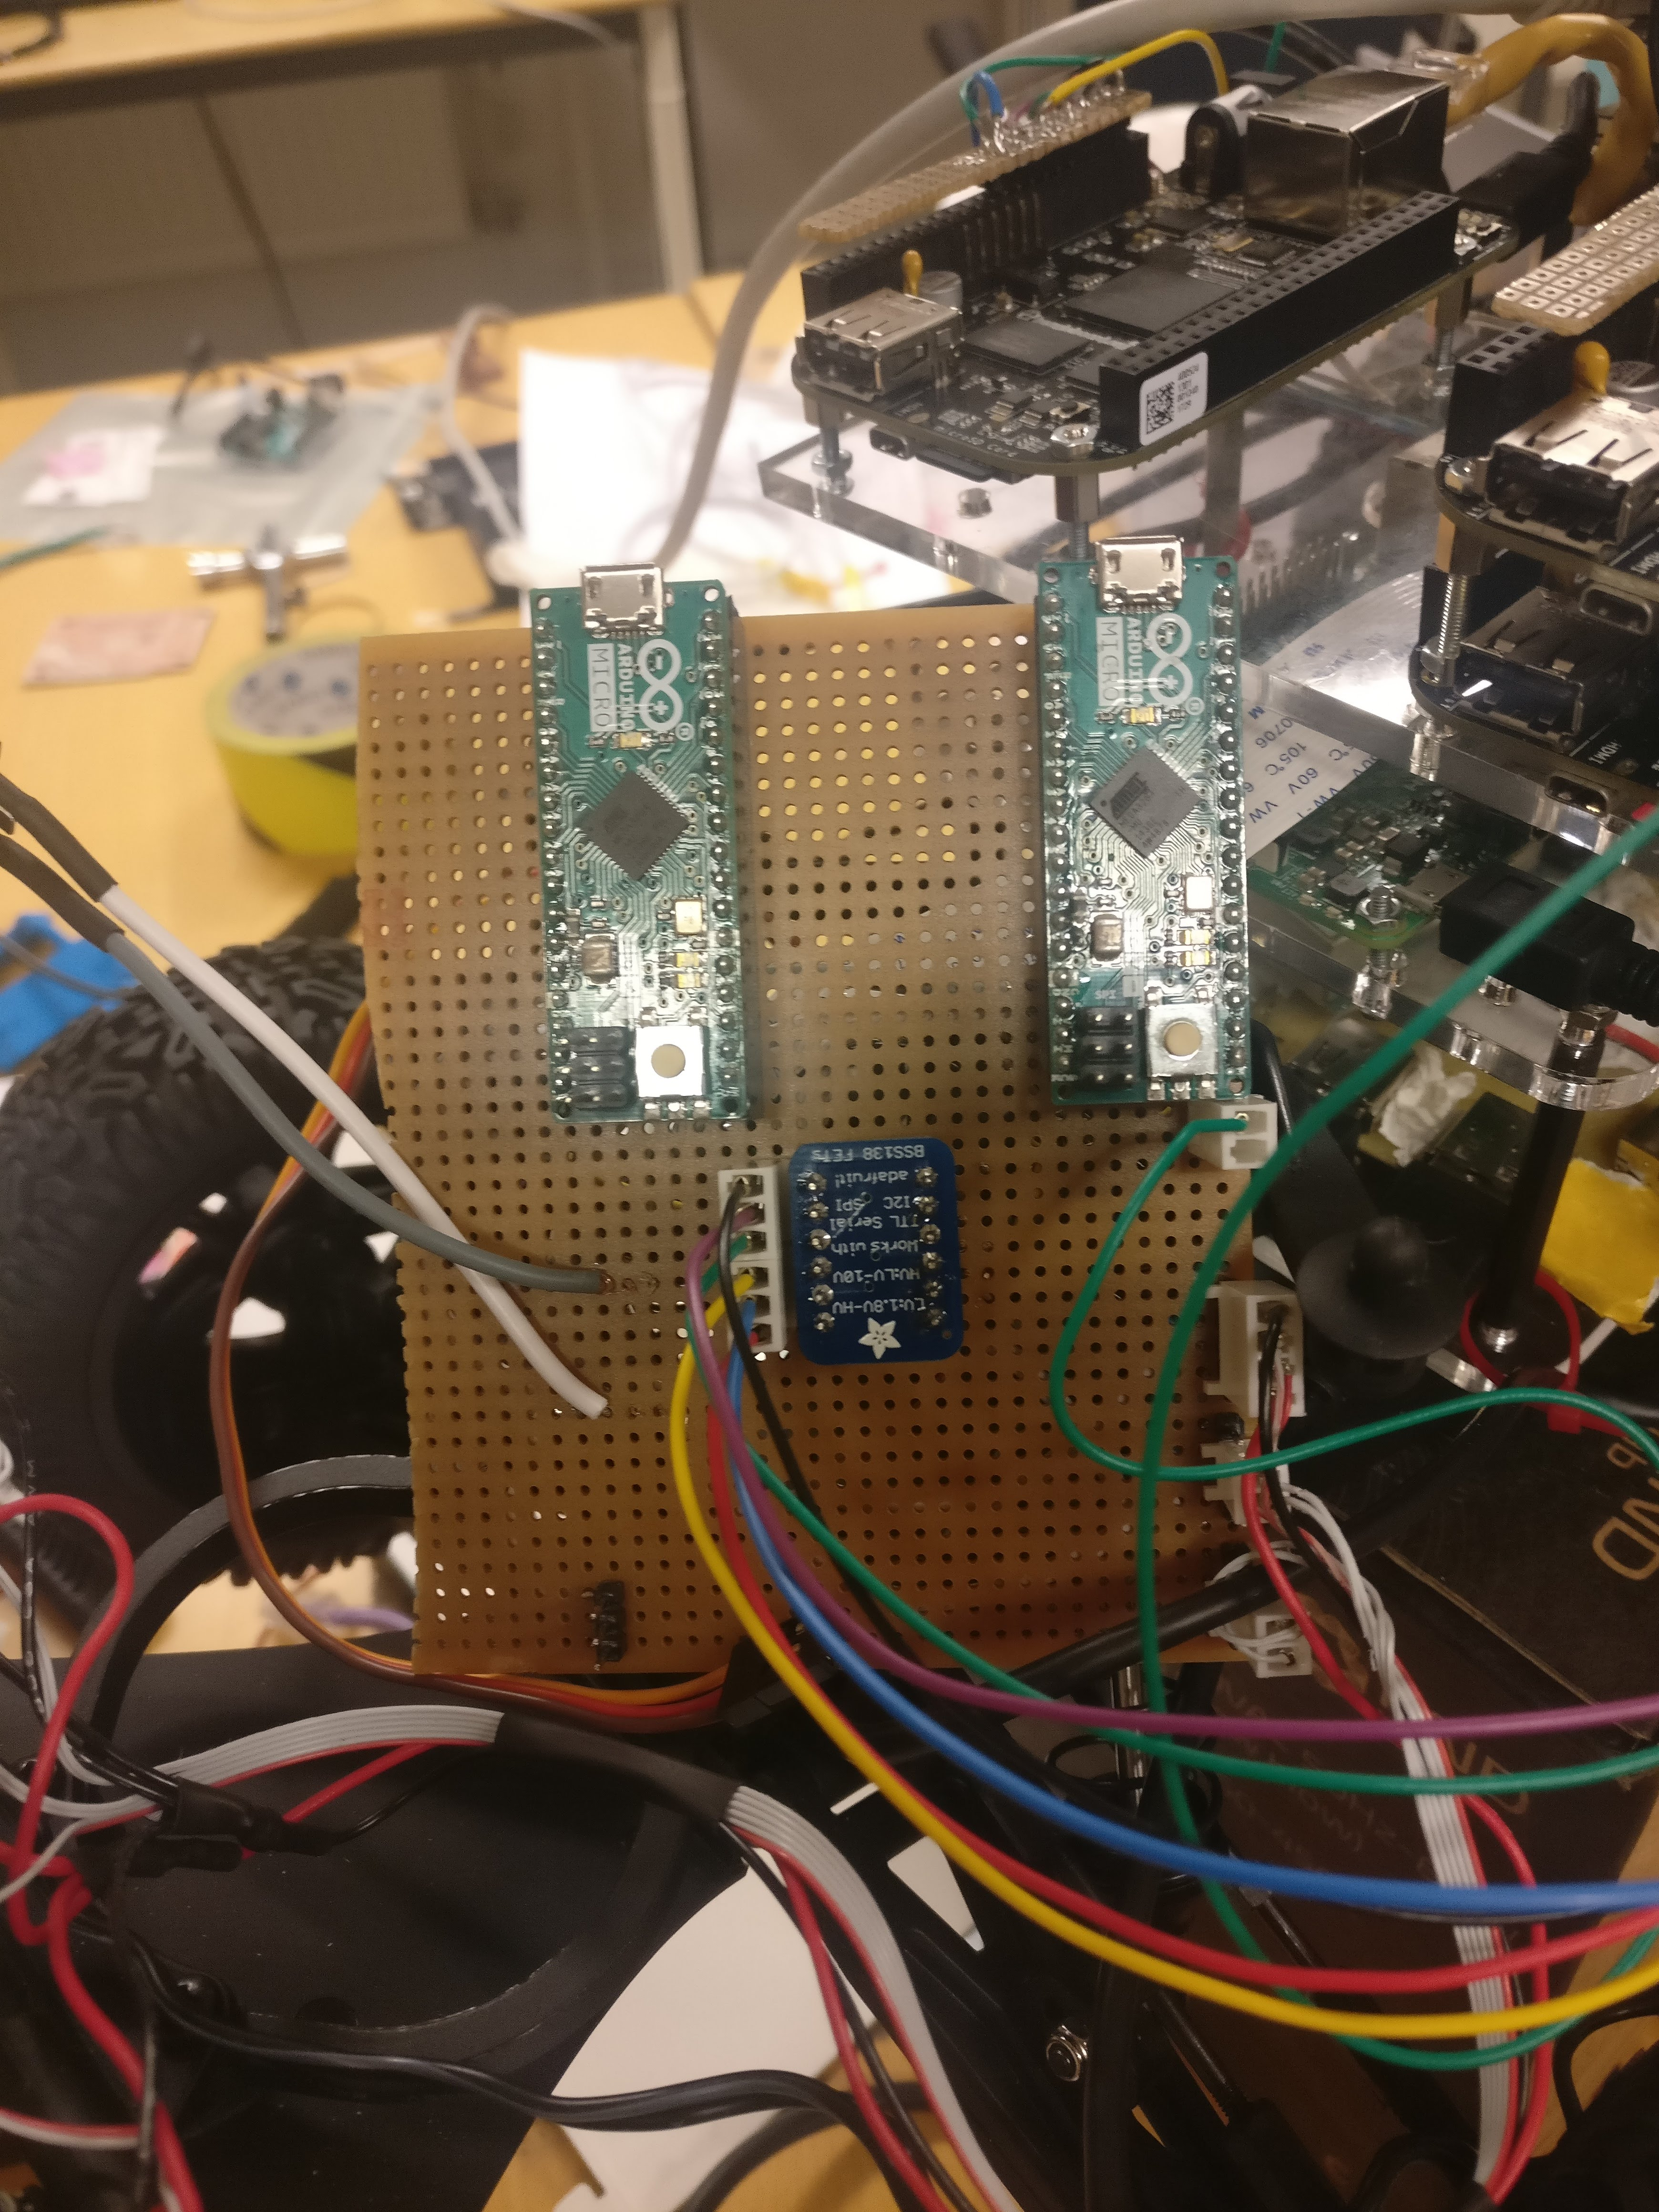
\includegraphics[width=0.3\textwidth]{arduino1.jpg}
	\caption{Arduino board for the steering and Ultrasound}
	\label{fig:board_ultra_steering}
\end{figure}

\begin{figure}
	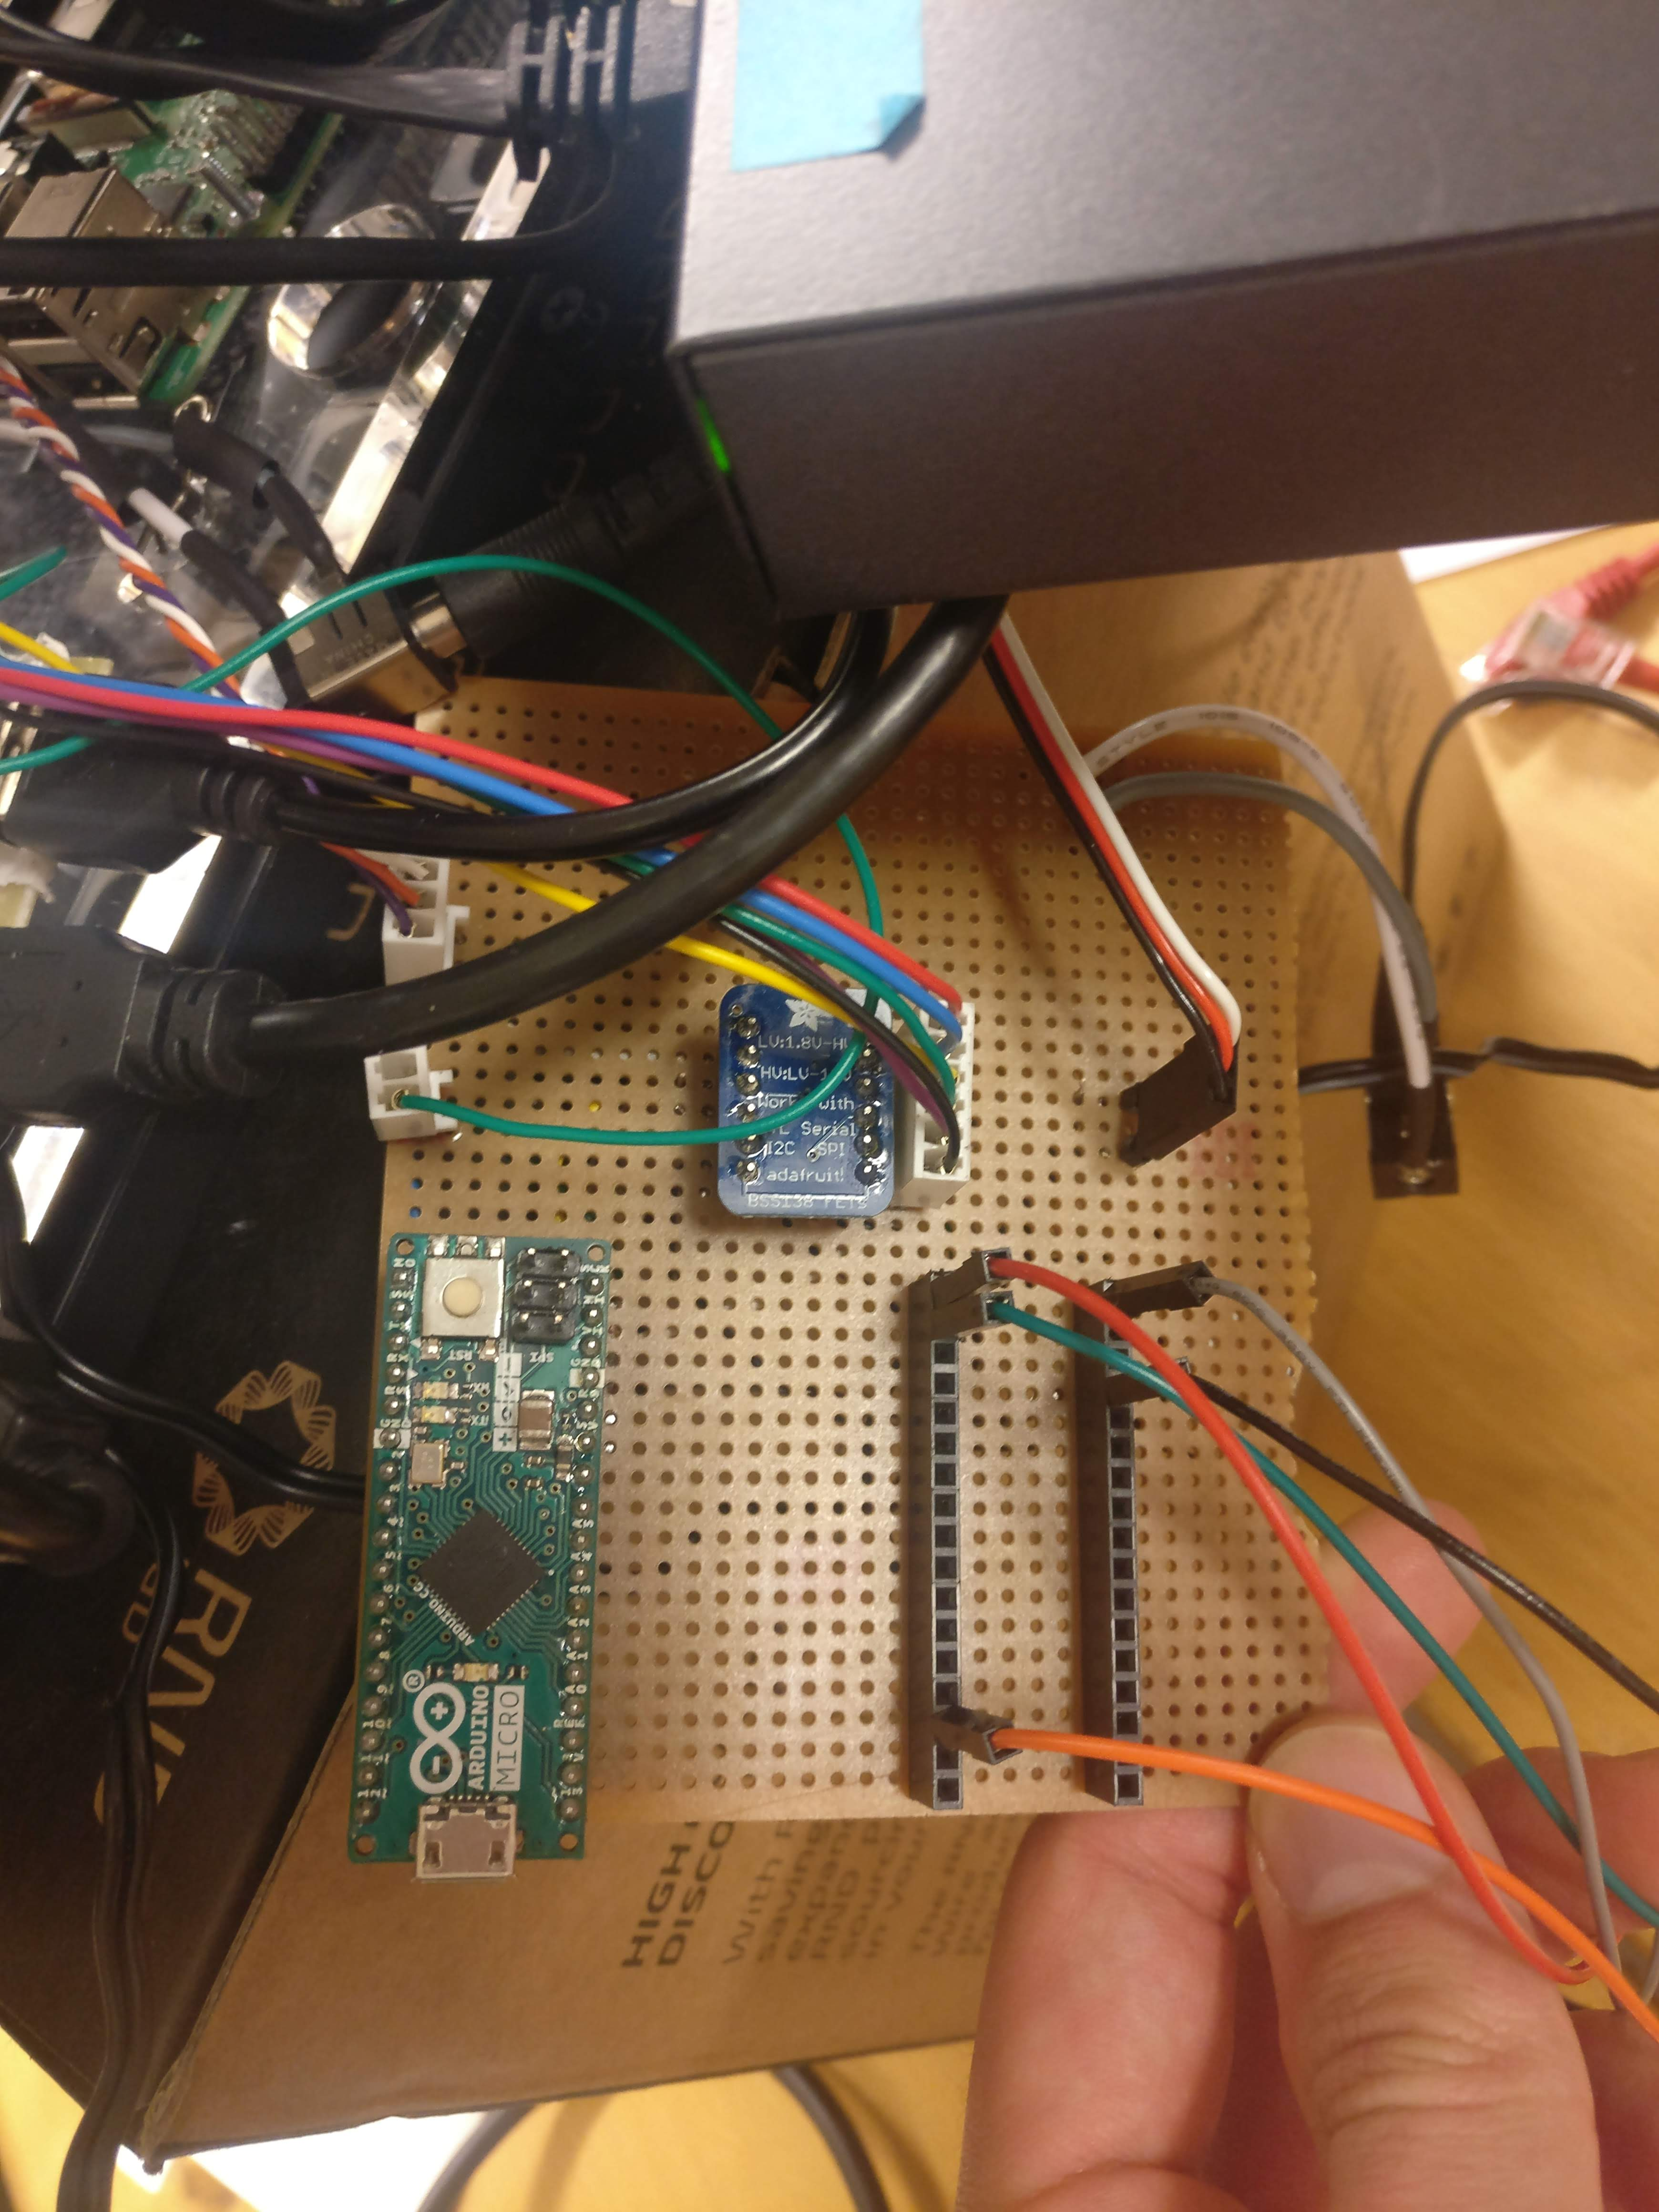
\includegraphics[width=0.3\textwidth]{arduino2.jpg}
	\caption{Arduino board for the engine and speed sensor}
	\label{fig:board_speed_engine}
\end{figure}

\begin{figure}
	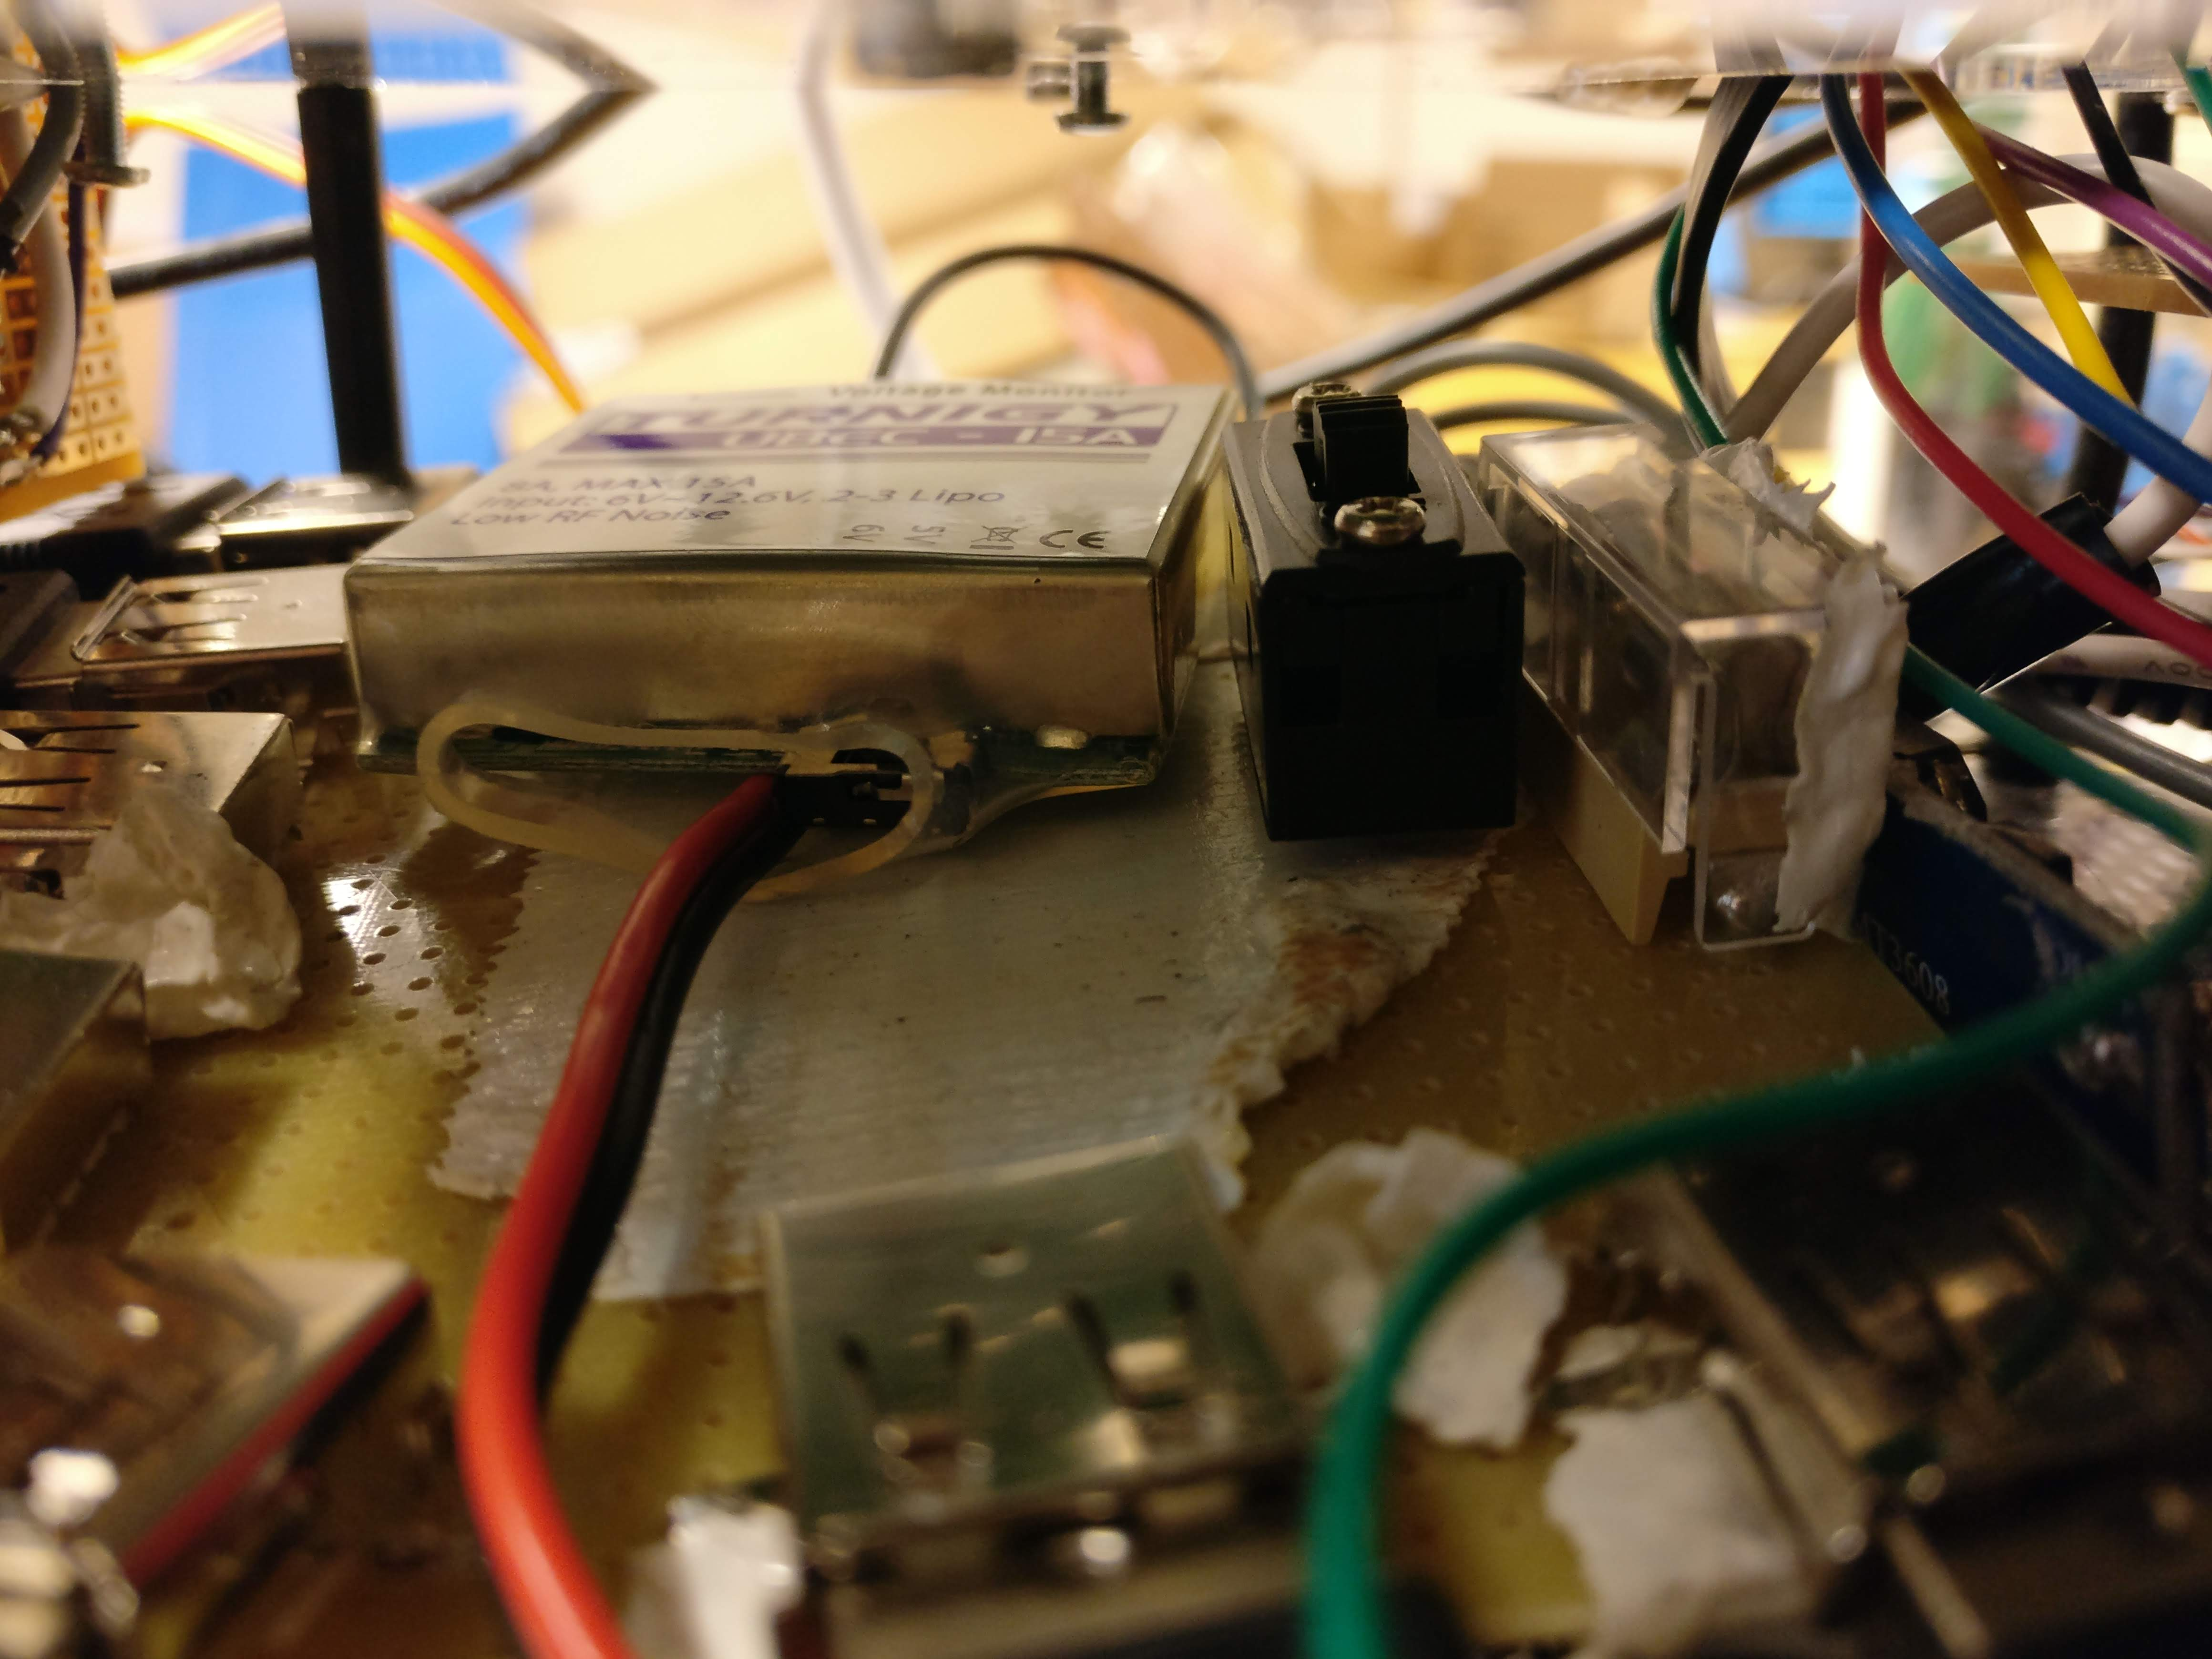
\includegraphics[width=0.3\textwidth]{power_board.jpg}
	\label{fig:Power_board}
	\caption{Power board}
\end{figure}



%-------------------------------------------------------------------------


\clearpage
\section{Verification and Validation}

\subsection{State machine}
The state machine was modelled and verified using the tool NuSMV which is a symbolic model checker that is used for formal verification of finite state systems. Since NuSMV allows for the models to be checked using linear temporal logic the state machine could be checked for node coverage and edge coverage. NuSMV also allows for exhaustive analysis meaning that each set of combinations of the state variables needs to have a defined behavioiur in each state of the model.

\subsection{Requirements and functionality}
The requirements and some of the system functionalities has been tested by following a set of test protocols and comparing the results with the expected outcomes. The protocols takes care of the communication between sensors and Arduinos, Arduinos and actuators, the SPI communication between Arduinos and BeagleBones, and the VSOME/IP packages to and from BeagleBones. The requirements tested was the ability to start the car, the flag following system, the collision avoidance system, and some of the fault states of nodes.

%TODO results
%-------------------------------------------------------------------------
\clearpage
\section{Results}

%-------------------------------------------------------------------------
\clearpage
\section{Discussion and Conclusion}

\subsection{Assembly and PCB}
Due course regulation was we not allowed to order PCBs from China and to order it from a European company was too expensive. 
The idea for the project was to design our own PCBs because the project should combine the knowledge we hade learned during our masters and some of the students in the project is taking the electronics track. But due to the course regulation were we not allowed to order from companies that did not accept invoice as a payment, it resulted that we could not order from the cheap PCB manufactures in China. The group tried to find a European company but they were too expensive. This lead to a redesign of the powering and we decided to use the milling machines but they there also broken so the only solution was to use prototype boards. There is kind of strange that there is no machines or ways to order PCB because the electronic track is to about design the electronics and there is no way for us to be able to satisfy the course goals. 

Because we hade to use prototyping boards and the platform was designed to have PCB mounted to it and not prototyping boards. This led to the assembly of the car was not as optimal as it could have been and the placement of come components and boards had to be placed at a different location. If the car would have been able to move around all it would have been affected of this, due the cable wiring was not optimal and the reliability of connections and wound have affected the car's performance. 


%-------------------------------------------------------------------------
\clearpage
\section{Future Work}
1.	The Pi camera can also output the distance, so that it can work as an alternative of the ultrasonic sensor. Since we are attempting to build a fault tolerant and self-adaptive system, we need the car be able to get the required data even when some sensors break down. Additionally, we can also take the distance into account when steering the car. For example, only when the distance from the car to the signal up to a specific value, the car start to follow the signal. Otherwise, it receive the signal but not carry out steering.
\newline
2.	Improve the communication between the color detection python code and VsomeIP, which causes some delay in our current version application. One possible solution is convert the python code into C++, so that the communication protocol will be simple and feasible.
\newline
3.	Although we have already tried to send the camera video stream to Android phone through WIFI so that we can directly see what the car is facing during running. We failed since the scripts of sending stream and color detection always block each other, it would be feasible to copy the video stream captured from Pi camera and one of them used as color detection, the other one can be sent to phone.
%-------------------------------------------------------------------------
\clearpage

\bibliographystyle{IEEEtran}

\bibliography{reference}
\clearpage
%-------------------------------------------------------------------------
\clearpage
%TODO appendix
\appendix
\clearpage

\end{document}
